\chapter{Background}\label{chapter:background}

% \Zeb{Argument of thesis is that it is important to explore the phonemic representation. In \cref{sec:12-inputrepresentations} I define ``input representation'', establishing a contrast between the default and phoneme input representation. Review past work on input representation in language models and recent work on tokenisation methods, concluding that the phoneme input representation is largely under-studied in the modern NLP landscape. In \cref{sec:12-phoneval} I review work regarding phonological evaluation of language models. This includes the use of the phoneme input representation in early connectionist models of language processing and computational models of acquisition as well as more recent work using phonemes in language models to study phonology cross-lingually to benchmarks that directly probe the phonological capabilities of LMs. Finally, in \cref{sec:12-babylm} I review work concerning the use of developmentally-plausible language models. Such models provide a useful framework for studying linguistic theories but mostly continue to use the default input representation, despite children not learning from arbitrary subwords. This chapter concludes that there is a clear need to study the use of the phoneme input representation in modern LM architectures.}

%CHAT: Language models (LMs) are systems that assign probabilities to sequences of linguistic units, such as words, characters, or phonemes. While architectural advances have received significant attention, the form of the input representation—how raw linguistic data is encoded for the model—remains a foundational and sometimes under-examined design decision. This chapter focuses on input representation, defined here as comprising three main components: modality (e.g. orthographic, phonemic), tokenisation, and pre-processing.
%Two major input paradigms are considered: subword-based input representations, which are now dominant in large-scale language modelling, and phoneme-based input representations, which provide an alternative aligned more closely with speech and cross-linguistic structure. Section 2 traces the historical development of input design choices across architectures. Sections 3 and 4 present each input paradigm in detail. Sections 5 and 6 examine their implications for phonological modelling and cognitive plausibility.
%A language model (LM) is a computational system that assigns probabilities to sequences of linguistic units, typically words, characters, or phonemes. Formally, given a sequence .. Language models can be used for generation, prediction, or as pre-trained components for downstream tasks. The input to a language model—referred to here as the input representation—is the focus of this chapter.

\defn{Language models} are statistical models of (natural) language that assign probabilities to sequences of linguistic units, such as words, characters or phonemes. While architectural advancements have received significant attention, the form of the \defn{input representation} --- how raw linguistic data is encoded for the model --- remains a foundational and under-examined design decision. Input representations are defined here as compromising three main components:

\begin{itemize}
    \item \textbf{Modality:} The modality of the raw data (e.g. orthographic text, phonemic transcriptions, audio).
    \item \textbf{Pre-processing:} Specific operations to clean the raw data, such as lowercasing or punctuation. 
    \item \textbf{Tokenisation:} How the pre-processed raw data is split into discrete tokens.
\end{itemize}

This thesis adopts a distinction between two broad types of input representation. The \defn{subword-based input representation} refers to the use of orthographic text, segmented into subword units, with whitespace-preserved word boundaries --- a representation that currently dominates large-scale language modelling. In contrast, the \defn{phoneme-based input representation} uses a phonemic modality for the raw data, removes explicit word boundaries and treats individual phonemes as atomic units. This representation has roots in computational models of language processing, speech recognition technology and phonological experimentation, but has rarely been examined in modern language model architectures --- the topic of this thesis.

This chapter provides the necessary background to understand the contrast between these paradigms. \Cref{sec:12-architectures} traces the historical development of input design choices across architectures. \Cref{sec:12-subword,sec:12-phonemic} present each input paradigm in detail. Finally, \cref{sec:12-plausiblepretraining} presents recent work in developmentally-plausible language modelling, a practical framework for exploring the use of a phoneme-based input representation with modern architectures.

\section{Evolution of input representations in language models}\label{sec:12-architectures}

% \Zeb{Insert figure comparing segmentations for tokenisation: character, subword, word, audio, maybe showing the shift over time.}

Instead of using a grammar to determine the structure of a sentence, language models are \emph{distributional} --- they assign probabilities to each linguistic unit in a sequence based on its context --- the ``company it keeps'' \citep{firth1957synopsis}. The standard formulation is:
\begin{align}
    P\left(w_t \mid w_1, \dots, w_{t-1} \right), \label{eq:languagemodel}
\end{align}

where $w_k$ denotes the linguistic unit at position $k$. These units are referred to as \defn{tokens} and are drawn from a set of possible tokens $\vocab$, also known as the \defn{vocabulary}. This formulation provides a convenient method for determining the probability of a sequence using the chain rule of probability:
\begin{align}
    P(w_1, \dots, w_T) = \prod_{t=1}^{T} P\left(w_t \mid w_1, \dots, w_{t-1}\right).
\end{align}


Language models of this type are called \defn{auto-regressive} since they predict the next item in a sequence based on on previous items from the same sequence, a principle first conceived by \citet{shannon1948mathematical}. This can be leverage in language generation tasks, where sequences can be produced by iteratively sampling from the distribution $P(\cdot | w_1, \dots, w_{t-1})$.

% TODO: Possibly insert XLNet and NAR below

In recent years, the term ``language model'' has also been used to refer to models do not use the language modelling equation above. For example, masked language models \citep[MLM;][]{devlin2019bert} are trained to predict items in a sequence using bi-directional context, but typically only in order to learn contextual representations of tokens for language understanding tasks, not to estimate probabilities or generate sequences. This thesis focuses on auto-regressive models, since the use of phoneme-based input representations is primarily explored in contexts where token-level or sequence-level probabilities are required.

The choice of input representation determines the manner in which the tokens represent natural language. %The tokenisation includes the granularity (e.g. words vs characters), the modality (e.g. phonemes vs graphemes) and whether pre-processing occurs.
The following sections explore how representations in language models have evolved alongside the development of new architectures and their emerging use cases.

\subsection{N-gram models}\label{sec:12-ngrams}

Early language models were \ngram models. Using a Markov chain of order $n-1$, these models provide an estimate of the next-token probability:
\begin{align}
    P\left(w_t \mid w_1, \dots, w_{t-1} \right) \approx P\left(w_t \mid w_{t-(n-1)}, \dots, w_{t-1}\right).\label{eq:ngram}
\end{align}

These probabilities are computed by calculating the frequency of \ngrams in a training corpus, where \ngrams are defined as contiguous subsequences of tokens of length $n$. Typically, these models use a word-based input representation: raw text is pre-processed with operations that may include lowercasing and accent stripping and then \textbf{tokenised} into word-like units. These operations are facilitated with libraries such as the Natural Language Tool Kit \citep[NLTK;][]{bird2009nltk}. 

Using word-level tokens is an intuitive choice for many NLP tasks, such as part-of-speech tagging, machine translation, text classification and language generation. Words naturally represent meaningful units in language and word-level predictions provide useful interpretations for these tasks. However, there are limitations to using words in \ngram models. One limitation is to do with their count-based nature. The number of possible \ngrams grows exponentially with $n$, making probabilities difficult to store and challenging to estimate due to sparsity. These models also struggle with rare words --- which Zipf's law states will inevitably appear \citep{zipf_human_1949} --- as well as with typos and other out-of-vocabulary (OOV) items, since they will not match any pre-computed \ngram probabilities. To mitigate sparsity and OOV issues, procedures such as Kneser-Ney back-off and Katz smoothing were developed \citep{ney1994structuring, katz2003estimation}, but the exponential factor means that \ngram models still struggle to scale beyond relatively small context windows.

Word-level tokenisation can also be a technical challenge. Early language model research focused on English, where using whitespace to create tokens for words and punctuations symbols is effective, but still requires special rules for dealing with clitics, contractions and compound words. In languages without clear word boundaries, dedicated systems are required to segment words, driven by NLP tasks such as Chinese Word Segmentation. Additionally, in morphologically rich languages such as Finish or Turkish, there is much higher word-form variation. For these languages, using \defn{morpheme-level} tokens addressed the resulting sparsity issues and increased generalisation, but required complicated systems to extract morphemes \citep{creutz2005unsupervised,habash2009}. % Possibly add something here about concept of a word being debated...

A lesser-used alternative to word-level tokens in \ngram models was to split sentences into individual \textbf{characters}. This reduces the vocabulary size considerably, allowing for slightly higher-order \ngrams to be computed, as well as providing a robust solution to OOV items. However, since words are split into many tokens, few syntactic dependencies are captured, limiting the utility of these models for many NLP tasks. Instead, these models were primarily used for character-sensitive tasks, such as spelling correction and auto-completion \citep{cucerzan_spelling_2004}.

$N$-gram models have also been used to model spoken language in tasks related to speech processing, including text-to-speech, accent recognition, language identification and automatic speech recognition (ASR). Instead of the raw data consisting of written text, these models use an input representation where tokens consist of individual \textbf{phonemes} --- the basic units of sound that distinguish words in spoken communication. Speech recognition systems often paired these phoneme-level language models with \textbf{acoustic models}, which map from acoustic features to phonemes as implemented in tool-kits such as HTK \citep{young2006htk}.

For many years, \ngram models were a cornerstone of NLP, providing the statistical backbone for early systems in translation and speech \citep{jurafsky2009speech}. They were used with a range of input representations, with tokens typically representing core linguistic units like words, morphemes, characters and phonemes, selected according to the downstream task. However, as neural architectures gradually replaced statistical language models across the NLP landscape, so too did the input representations leveraged by these models.

\subsection{Neural language models}

Neural language models began with the work of \citet{bengio2003neural}, who used a feed-forward neural network to predict the next word given a fixed-length context. This approach addressed the sparsity and poor generalisation of \ngrams by learning distributed word embeddings, but remained limited in both context size and computational efficiency. The transition to more effective neural architectures was driven by advances in representation learning --- most notably Word2Vec \citep{mikolov_distributed_2013} --- and by the adoption of recurrent neural networks (RNNs) for language modelling \citep[RNNLMs;][]{mikolov2010recurrent}, which offered the ability to model sequences with theoretically unbounded context. In practice, however, RNNs struggled to capture long-range dependencies due to the \emph{vanishing gradient problem}, which caused the influence of earlier tokens to diminish over time. This limitation was addressed by long short-term memory networks \citep[LSTMs;][]{sundermeyer2012lstm}, which introduced gating mechanisms to help retain relevant information across longer spans. 

Many of these early recurrent networks still operated at the word-level, using a dedicated unknown token \texttt{<unk>} for rare words, and either learned word embeddings during training or used pre-trained embeddings from systems like Word2Vec or GloVe \citep{pennington2014glove}. This word-level granularity was well-suited to the relatively small vocabularies and modest training corpora of the time, but the limitations associated with word-level representations persisted: out-of-vocabulary (OOV) words were common and rare words had poorly estimated representations, causing generalisation issues particularly for morphologically-rich languages. Some work has explored character-level or morpheme-level inputs to address these issues \citep{botha2014compositional, jozefowicz2016exploringlimitslanguagemodeling, kim2016character, vania2017morphology, gerz2018, ustun-etal-2018-characters} often by composing word embeddings from these granular units using convolutional or recurrent architectures.

\begin{table*}[t]
    \centering
    \small
    \addtolength{\tabcolsep}{-0.2em}
    \begin{tabular}{lc}
        \toprule
        \textbf{Granularity} & \textbf{Example} \\
       \midrule
        Word-level & ~\mybox{molecules} ~\mybox{are} ~\mybox{unstable} \\
        Subword-level & ~\mybox{m} ~\mybox{ole} ~\mybox{cules} ~\mybox{Ġare} ~\mybox{Ġunstable} \\
        Morpheme-level & ~\mybox{molecule}~\mybox{s} ~\mybox{are} ~\mybox{un} ~\mybox{stable} \\
        Character-level & \mybox{m} ~\mybox{o} ~\mybox{l} ~\mybox{e} ~\mybox{c} ~\mybox{u} ~ \mybox{l}~ \mybox{e}~ \mybox{s}~ \mybox{\textvisiblespace} ~ \mybox{a}~ \mybox{r}~ \mybox{e}~ \mybox{\textvisiblespace}~ \mybox{u}~ \mybox{n}~ \mybox{s}~ \mybox{t}~ \mybox{a}~ \mybox{b}~ \mybox{l}~ \mybox{e} \\
        Phoneme-level & \mybox{\textipa{m}} ~\mybox{\textipa{A}} ~\mybox{\textipa{l}} ~\mybox{\textipa{I}} ~\mybox{\textipa{k}} ~\mybox{\textipa{u:}} ~ \mybox{\textipa{l}}~ \mybox{\textipa{z}}~ \mybox{\textipa{A}}~ \mybox{\textipa{\*r}} ~ \mybox{\textipa{2}}~ \mybox{\textipa{n}}~ \mybox{\textipa{s}}~ \mybox{\textipa{t}}~ \mybox{\textipa{eI}}~ \mybox{\textipa{b}}~ \mybox{\textipa{@}}~ \mybox{\textipa{l}} \\
        \bottomrule
    \end{tabular}
    \caption{A comparison of granularity levels in tokenisation using the phrase ``molecules are unstable''. The BPE tokeniser used to train \gpt\textsuperscript{1} is used for the subword-level tokens, where `Ġ' is the dedicated prefix for word-initial tokens. `\textvisiblespace' is used to denote the space character.  Phoneme-level tokenisation is similar in granularity to character-level tokenisation but word boundaries are removed, and when using the International Phonetic Alphabet, some phonemes consist of multiple characters.}
    \label{tab:12-granularity}
    \vspace{-4mm}
\end{table*}

A more scalable solution emerged in the form of Byte Pair Encoding (BPE), originally proposed as a compression method by \citet{gage1994new} but introduced to NLP in the context of neural machine translation by \citet{sennrich-etal-2016-bpe}. BPE offers a data-driven, unsupervised algorithm that begins with character-level tokens and iteratively merges the most frequent adjacent pairs into longer units, balancing vocabulary size with the ability to represent rare and unseen words. These units are typically called \defn{subwords}, which can consist of entire words or individual characters. Their granularity lies somewhere between words and characters, as shown in \cref{tab:12-granularity}, but they are not linguistically grounded. Subword-based representations are discussed in more detail in \cref{sec:12-subword}.\footnotetext[1]{\href{huggingface.co/openai-community/gpt2}{https://huggingface.co/openai-community/gpt2}}

%Unlike word-level models, BPE allows open-vocabulary modelling while retaining frequent words as atomic units, enabling better generalisation across morphological variants without relying on handcrafted segmenters. Its efficiency, simplicity, and language-agnostic design made it a de facto standard in subword tokenisation, especially in recurrent and early Transformer-based architectures.

Despite the advantages of subword tokens, using shorter tokens creates longer sequences, and despite capturing long-distance dependencies, LSTMs still process data sequentially and so struggle to learn compositional meaning across distant tokens. This meant that these more granular input representations remained secondary to word-level modelling, until the advent of the transformer.

\subsection{Transformers and the shift to subword units}

Transformers \citep{vaswani2017attention} addressed many of the limitations that made subword tokenisation challenging for LSTMs. Instead of sequential processing, transformers rely entirely on self-attention mechanisms that allow them to access all positions in the input simultaneously. By better facilitating the modelling of long-range dependencies, transformers are better equipped to compose meaning from longer sequences of subword units. 

There are considerable variations of these architectures, with \myemph{GPT} \citep{radford2018gpt1} and \bert \citep{devlin2019bert} as foundational models, both of which used a subword-based input representation. GPT models are auto-regressive, trained with the language modelling objective, whereas \bert-style models use the MLM objective to benefit from bi-directional context. Transformer-based language models quickly began to out-perform past approaches across most NLP tasks, establishing subword units as the default input representation in modern large-scale language models. These architectures are now so ubiquitous that the term ``language model'' without further disambiguation invokes them implicitly. As such, the acronym LM will henceforth be used to refer to transformer-based autoregressive language model in this thesis.

Although there have been many attempts to integrate character-level or morpheme-level information when training LMs \citep[e.g.][]{ma-etal-2020-charbert, nzeyimana-niyongabo-rubungo-2022-kinyabert}, subword-based encodings have remained the default. This is primarily because subwords efficiently address the trade-off between vocabulary size and sequence length; whereas number of embeddings grows linearly with the vocabulary size, making more granular encodings desirable, inference scales \emph{quadratically} with the context size due to the self-attention mechanism. Subwords thus not only provide generalisability, but avoid large vocabulary sizes without creating overly long sequences, particularly when using compression-driven methods like BPE. Although morphological tokenisation also seems to address this trade-off while providing a more linguistically-motivated unit (as shown in \cref{tab:12-granularity}), mapping orthographic text to morphemes continues to be a challenging task, often requiring dedicated systems trained on labelled corpora \citep{batsuren-etal-2022-sigmorphon}. 
%\zeb{Maybe need to mention MAMBA somewhere.} 

Despite subwords becoming the default tokenisation scheme, other aspects of the input representation continued to be tailored for specific domains. For instance, models based on the \bert architecture were trained to provide better encodings of biomedical literature \citep[\myemph{BioBERT};][]{lee2020biobert}, legal text \citep[\myemph{LEGAL-BERT};][]{chalkidis2020legal}, clinical notes \citep[\myemph{Clinical BERT};][]{alsentzer2019publicly} and programming languages \citep[\myemph{CodeBERT};][]{feng-etal-2020-codebert}. By using specific pre-processing steps and vocabularies, these models achieved better performance on tasks related to these domains.

Pre-processing practices were also driven by computational considerations. Subword-based representations have a vocabulary of single-character units as a fall-back, but the number of unique characters in schemes like UTF-32 is enormous. \bert addressed this using unicode normalization (e.g. NFD normalisation replaces \ex{\'e} with \ex{e\'{}}) whereas later models follow \gpt \citep{radford-2019-gpt2} in mapping characters to a byte-level vocabulary before splitting into subwords, a process that can then be reversed during decoding \citep{wang2020neural}.  

The advent of large language models (LLMs) has significantly reduced the emphasis on carefully tailored input representations. Rather than training separate models for individual downstream tasks, current practice centres on pre-training a single, general-purpose model on massive text corpora. These models can then be adapted to a wide range of applications through fine-tuning or even used directly in zero-shot or few-shot settings \citep{raffel2020exploring}. This shift has motivated the use of a consistent, task-agnostic input representation, as empirical findings suggest that scaling up data yields greater performance gains than carefully tuning tokenisation or pre-processing pipelines \citep{brown-2020-gpt3}. 

To match their growing capacity, LLMs require vast quantities of training data, much of which is sourced through web-scraping \citep{bansal-2022-datascaling}. Such data is inherently noisy, which has driven a shift toward scale, architecture and data-driven tokenisation methods rather than linguistic heuristics. Indeed, noise in training data has been shown to improve generalisation \citep{zheng-saparov-2023-noisy}, further diminishing the need for elaborate pre-processing. As a result, modern tokenisers typically apply minimal pre-processing. The sheer scale of these models --- often trained on trillions of tokens and containing billions of parameters --- has dramatically increased computational demands, leading to significant financial and environmental costs \citep{strubell-etal-2019-energy, patterson2021carbonemissionslargeneural, bender2021parrots, luccioni2022estimatingcarbonfootprintbloom}, further causing computational considerations to outweigh other factors when it comes to selecting the input representation. 

% CHAT: This shift reflects confidence in model capacity and a preference for data-driven robustness, reducing reliance on linguistic heuristics.

Model capacity and architectural advances have also impacted the input representations used for models operating in the audio modality. Instead of creating systems that combine acoustic models with phoneme language models, recent advances have demonstrated that representations can be learned directly from raw waveforms or spectrograms --- with Wav2Vec \citep{baevski2020wav2vec}, \myemph{HuBERT} \citep{hsu2021hubert} and Whisper \citep{radford2023robust} as notable examples. However, these systems require substantially more data than previous methods, which can limit their use in low-resource settings, as discussed in \cref{sec:12-practicalphoneme}. Audio-based representations are further considered in contrast to phoneme-based representations in \cref{chapter:discussion}.

Consequently, whereas past models typically used linguistically-motivated representations curated for a specific task, the primary motivators for input representations in the modern NLP landscape are generalisability and computational efficiency. These have led to subword-based representations becoming the norm in the text-based domain. These data-driven methods are also easier to apply to noisy datasets than linguistically-motivated methods. In the audio domain, increased model capacity had led to representations being learned directly from audio. Hence, the use of phoneme-based representations remains under-explored. 

% ADD \citep{zellers-etal-2019-hellaswag, hendrycks-2020-mmlu, suzgun-2023-Big-Bench}.?

\subsection{Small language models and a return to domain-specific pre-training}\label{sec:12-domainspecific}

In recent years there has been a shift away from the LLM paradigm back towards the training of smaller LMs. At the time of writing, `small' LMs  refer to models with significantly fewer parameters than their LLM counter-parts, typically ranging from tens to a few hundred million parameters --- similar in scale to the original \bert and GPT models. There are several motivations for this shift to small LMs, three of which are considered below; computational constraints, over-generalisation and linguistic research.

\paragraph{Computational constraints.} The LLM paradigm focuses on training very large models on a broad range of data (often including multilingual data and code) that then be fine-tuned for specific tasks or applications. For example, the open-sourced \llama-3 suite of models range from 8B to 405B parameters and when fine-tuned, achieve state-of-the-art results on benchmarks across a broad range of categories including mathematics, language understanding, code generation and multilingual modelling \citep{grattafiori2024llama}. However, this paradigm makes pre-training research outside of industry infeasible (the largest Llama-3 model was trained on up to 16K GPUs).

Instead, smaller LMs are used as proxies for studying architecture \citep{charpentier2024gpt}, training dynamics \citep{martinez2024tending} or data curation strategies \citep{huebner-etal-2021-babyberta}. While they cannot match the capabilities of frontier-scale models, findings from small-scale experiments can still yield valuable insights. Often, these studies explore models across scales, which is important due to the fact that certain emergent behaviours only appear at larger model sizes \citep{wei2022emergent, ganguli2022predictability}. For example, the Pythia suite provides models ranging from 14M to 12B parameters, along with training checkpoints, specifically to enable the analysis of LM across training and scales \citep{biderman2023pythia}.

The fine-tuning paradigm itself also has computational constraints. The common understanding is that fine-tuning is both cheaper than pre-training a new LM from scratch and that the resulting model benefits from the language understanding capabilities gained from these massive pre-training efforts. However, LLMs have become so large that even efficient fine-tuning strategies like Low-Rank Adaption \citep[LoRA;][]{hu2022lora} can still be computationally demanding. For example, \citet{fittschen2025pretraininglanguagemodelsdiachronic} compared pre-training small LMs (345M parameters) to fine-tuning \llama-3 (8B parameters) for a set of diachronic linguistics tasks. They found that not only was pre-training cheaper than fine-tuning, but that the smaller LMs yielded better detection of language change and word sense introduction/obsolescence. 


%\zeb{Here, possibly insert work on challenges of continual pre-training or fine-tuning for domain adaptation}
\paragraph{Over-generalisation.} The assumption that large generalised models are well-suited for domain-specific tasks has been increasingly questioned. For instance, in their study, \citet{fittschen2025pretraininglanguagemodelsdiachronic} hypothesised that the fine-tuned \llama-3 underperformed because its pre-training on modern language introduced systematic biases --- effectively `leaking' contemporary linguistic features into a task requiring temporal specificity. Similar concerns arise in the multilingual setting, where multilingual LLMs often exhibit a strong bias towards English \citep{wendler-etal-2024-llamas}. \llama-3, for instance, was trained on a total of 15T multilingual tokens, yet only 8\% of this data represents the 176 non-English languages in its corpus.\footnote{A further 25\% of the corpus represents mathematical reasoning and 17\% represents code.} The ratio of English to multilingual data was tuned experimentally with equal weight given to English performance as multilingual performance \citep{grattafiori2024llama}, demonstrating this bias. The common belief that LLMs can leverage transfer learning to support the modelling of low-resource languages has been thoroughly explored \citep{wu-dredze-2019-beto}. The ``curse of multilinguality'' predicts performance degradation for low-resource languages due to model capacity \citep{conneau2020unsupervised}. \citet{chang2024goldfish} report that for many low-resource languages, multilingual LLMs exhibit higher perplexity than even simple bigram models. Their Goldfish suite of models consists of monolingual models across 250 languages, some of which, trained on as little as 5MB of data, out-perform multilingual LLMs. Similarly, \citet{chang2024multilinguality} show that while multilingual data can sometimes help low-resource modelling, excessive multilingual pre-training may degrade performance for both low- and high-resource languages. Whether in diachronic linguistics or under-resourced language settings, these findings represent a return to domain-specific pre-training with suggestions that smaller, purpose-built models can outperform large-scale LLMs in certain cases.

\begin{figure}
    \centering
    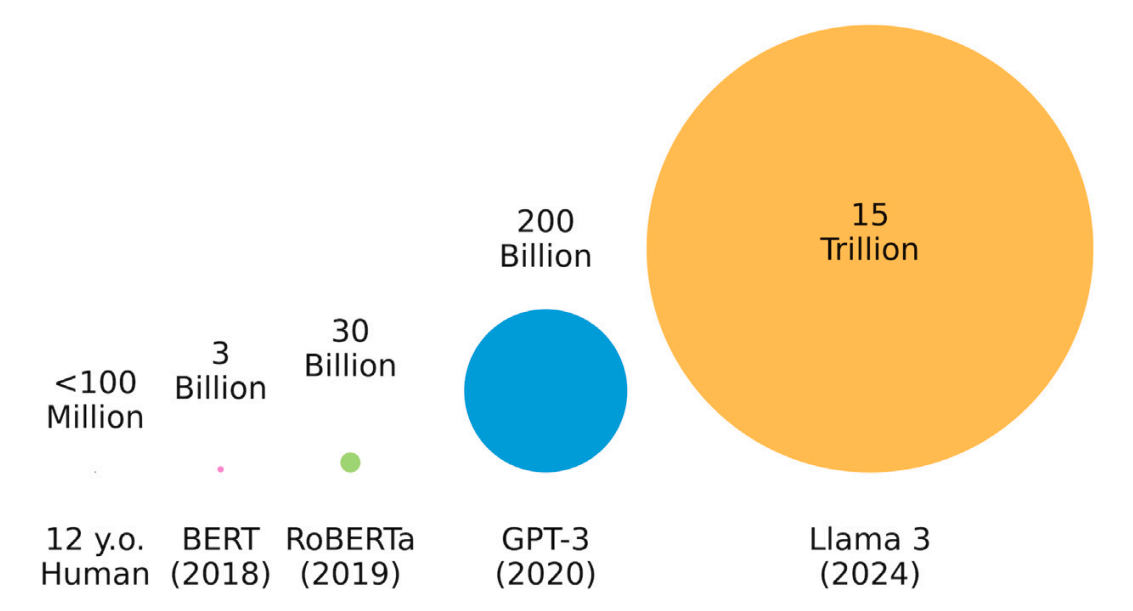
\includegraphics[width=0.99\linewidth]{12Background/scales.png}
    \caption{Mainstream language models are trained on multiple orders of magnitude more word tokens than the amount available to a typical child. \emph{Reproduced from \citet{wilcox2025bigger} under CC BY 4.0.}}
    \label{fig:12-scales}
\end{figure}

\paragraph{Linguistic research.} For decades, language models have been used to study human language learning and processing. For example, \citet{hale-2001-probabilistic} introduced surprisal theory, establishing a groundbreaking connection between the negative log-probability of a word (according to a language model) and real-time human language processing. This finding has been demonstrated repeatedly in ever-more sophisticated language models architectures, correlating surprisal with reading times, eye movements and brain activations \citep[e.g.][]{levy2008expectation, futrell2019neural, futrell2020lossy, schrimpf2021neural}. Early demonstrations that connectionist models can learn grammatical patterns from data alone \citep[e.g.,][]{elman-1990-finding, macdonald1994lexical} revived foundational questions about the \emph{learnability} of natural language \citep{gold1967language}. The increasing capabilities of language models and their success on downstream tasks has motivated research into the internal representations of LMs and assessing their ability to learn human-level grammatical generalisations \citep{hewitt-manning-2019-structural, hu-etal-2020-systematic, manning-2020-emergent}.

However, there are issues with using LLMs for testing probabilistic theories of language processing. Considering surprisal theory, \citet{wilcox2020predictive} found that language models with a better ability to predict upcoming words are also better predictors of human language processing. However, \citet{shain2024large} and \citet{oh2024frequency} found that this trend is reversed in LLMs. \citet{wilcox2025bigger} argue that ``bigger is not always better''; LLMs are now such good predictors of language that they no longer provide human-like probability distributions that can be used to further psycholinguistic theories. This is also the case for using LLMs as cognitive models of human language learning. Researchers that advocate for the use of language models as cognitive models highlight the importance of human-like pre-training with a particular focus on the \emph{scale} of data used to train these models \citep{linzen-2020-accelerate,baroni-2022-proper,warstadt-2022-artificial,wilcox2025bigger}. This is illustrated in \cref{fig:12-scales}, which shows that \llama-3 is exposed to hundreds of thousands of times more words than the what humans experiences by the onset of adolescence --- estimated to be 100M words for children growing up in the United States \citep{gilkerson2017mapping}. Besides scale, there are also concerns that the domain of pre-training data is not developmentally plausible \citep{huebner-etal-2021-babyberta, warstadt2023findings} and that using input representations that do not resemble the sensory signals perceived by humans during language learning confound possible insights gained from using language models as cognitive models \citep{dupoux-2018-cognitive}. 

%However, underlying these approaches is a concern that language models trained under common paradigms may not be scientifically sound for providing insights into human language acquisition. This is because the development of language models is driven by downstream performance on popular tasks rather than being grounded in linguistic theories \citep{baroni-2022-proper}. The recent explosion in the size of language models has further complicated comparisons between human and neural network language acquisition. \citet{warstadt-2022-artificial} argue that to draw valid conclusions about human language acquisition from neural networks, the trained models should not possess any advantages over humans. Similarly, \citet{dupoux-2018-cognitive} proposes that machine learning models should use raw sensory signals perceived by humans (e.g., sound waves) as inputs to remove confounding variables that make interpreting their behaviour as models of language acquisition challenging. Similarly to how the BabyLM challenge reduces the training set to a reasonable size, the Zero Resource Speech Challenge involves developing unsupervised methods that learn language directly from audio \citep{dunbar_self-supervised_2022}. We discuss this paradigm further in \cref{sec:14-audiomodels}.

Motivated by these concerns, the BabyLM challenge was developed to encourage pre-training research with developmentally-plausible corpora \citep{warstadt2023findings, hu-etal-2024-findings}. Participants are challenged to train small LMs on a corpus of 100M words, using speech transcripts and child-directed domains as source data. However, the challenge uses textual data, and the vast majority of participating systems use subword-based input representations. There are similar communities that focus more on the plausibility of the input representation, such as the Zero Resource Speech Challenge, which promotes developing unsupervised methods that learn language directly from audio \citep{dunbar_self-supervised_2022}. This work is discussed further in \cref{chapter:discussion}.

\paragraph{} The three factors discussed above have contributed to the recent shift toward training smaller language models in domain-specific and developmentally-plausible settings. Yet, within this work, comparatively little attention has been paid to the input representations used by these models. The computational and architectural pressures that originally motivated the adoption of subword units have become so dominant that most research now focuses on variations of subword tokenisation methods, rather than exploring alternative forms of representation, as discussed in \cref{sec:12-subword}.

The BabyLM challenge exemplifies how entrenched subword-based input representations have become. Although concerns about developmental plausibility might naturally encourage the use of auditory or visual representations --- such as the phoneme-based inputs used in early cognitive models (see \cref{sec:12-phonemic}) --- the subword-based representation is the default. The organisers acknowledge that this is a limitation of the framework \citep{wilcox2025bigger}, pointing to both the lack of suitable alternative data and an aim to attract broader participation as reasons for this choice. Indeed, the challenge is motivated not only by the goal of advancing cognitive and psycholinguistic modelling, but also by more practical objectives such as democratising pre-training research and accelerating architectural innovation --- goals for which text-based subword representations are well suited. Nonetheless, developmentally-plausible pre-training remains a promising framework for exploring phoneme-based input representations, as discussed further in \cref{sec:12-plausiblepretraining}.

%However, they do not address the other developmental concern, that the subword-based representation may not be appropriate for this line of research --- in part, this is because these representations have become so standardised that they feared losing participants by exploring more plausible domains (see \citet{wilcox2025}). Additionally, the challenge also has wider goals of democratising LM research and exploring data-efficient pre-training methods, which could clash with using a developmentally-plausible input representation.

\section{Subword-based input representation}\label{sec:12-subword}

Modern large language models (LLMs) that operate on textual input rely on subword-based input representations, which offer a balance between generalisability and computational efficiency. In the standard framework, the conversion from raw text to model-ready input is handled by a component known as a \defn{tokeniser}, as implemented in libraries such as \texttt{HuggingFace Tokenizers}.\footnote{\href{https://huggingface.co/docs/tokenizers/index}{huggingface.co/docs/tokenizers/}} A typical tokenisation pipeline comprises several sequential stages:

\begin{itemize}
\item \textbf{Pre-processing:} Operations such as lowercasing, accent removal, Unicode normalisation, or character-to-byte conversion.
\item \textbf{Pre-tokenisation:} Splitting the input into word-like units, often using whitespace and punctuation.
\item \textbf{Subword model:} Segmenting word-like units into subword tokens using models such as BPE, WordPiece, or Unigram.
\item \textbf{Vocabulary mapping:} Converting subword tokens into integer IDs for input to the model.
\item \textbf{Post-processing:} Adding special tokens required by the model (e.g. \texttt{<BOS>}, \texttt{<EOS>}, or segment markers).
\end{itemize}

This pipeline broadly mirrors the classical NLP approach to text processing, although some terminology has shifted: what was once referred to as ``tokenisation'' is now more precisely termed ``pre-tokenisation''. However, due to the centrality of subword segmentation in modern architectures and minimal pre-processing practices, the terms ``tokenisation'' and ``tokeniser'' have become overloaded. In their narrow sense, they refer specifically to the operations of the subword tokenisation model. In their broader sense, they encompass the entire pipeline from raw text to token IDs.

In this thesis, the terms ``subword tokenisation'' and ``subword tokeniser'' will be used to refer to the narrow sense, while ``tokenisation'' and ``tokeniser'' will be used in the broader sense unless otherwise specified.

% Packaging up these pre-processing steps into a single tokenizer provides convenience, but this has had consequences. In classical NLP, it was an important step to carefully considering the data cleaning operations. For example, removing punctuation... \writemore. The scaling ability of modern LMs has largely shifted the focus to language model architectures and machine learning algorithms, with many models using default tokenisers from Huggingface without considering the impact. This is particularly the case for studies using smaller LMs to study language or acquisition (see \cref{sec:12-babylm}) where subwords in particular may not be an appropriate base unit, nor the orthographic domain if simulating spoken speech. In these cases the default representation is no longer as crucial for performance, yet the convenience of the existing frameworks facilitates its use. 

% The design and availability of this tokenization pipeline has largely been driven by the sheer scaling capabilities of LM architectures, the largest of which are called ``large'' language models (LLMs). Now, the vast majority of language models are distributed on platforms such as Huggingface with an associated tokenizers that consistently process orthographic text, pre-tokenize the text to preserve word boundaries, and return tokens representing subwords.

\subsection{Subword tokenisation methods}\label{sec:12-subwordmethods}

Formally, subword tokenisers can be defined as a tuple $\tokeniser \defeq (\vocab, \detok, \tok)$. The first item in the tuple is the \defn{vocabulary} $\vocab$: a finite set of subwords, each defined as a concatenation $\subword \defeq \ch_i \circ \cdots \circ \ch_j$ of symbols $\ch$ from an alphabet $\alphabet$. The alphabet can be defined as set of characters appearing in the pre-tokens --- this can be all unique characters appearing in the data (e.g. letters, punctuation and whitespace) or the set of all bytes, if using character-to-byte conversion. %Without loss of generalisation, the alphabet is assumed to be bytes below.

The remaining components are two functions that map between symbol sequences and subword sequences: the \defn{detokenisation function} $\detok\colon \vocab^* \to \alphabet^*$ reconstructs a symbol sequence from subwords, by concatenating subwords; the \defn{tokenisation function} $\tok\colon \alphabet^* \to \vocab^*$ performs the reverse mapping and must be injective, satisfying $\chvec = \detok(\tok(\chvec))$.

A common class of subword tokenisers are \defn{bottom-up tokenisers}. These tokenisers choose their vocabulary sequentially, starting from an initial set of symbols (e.g., bytes) and iteratively merging pairs of symbols until a pre-specified vocabulary size is achieved. For example, BPE \citep{gage1994new,sennrich-etal-2016-bpe} and WordPiece \citep{schuster-nakajima-2012-voice} are two popular instances of this class.

Training a tokeniser amounts to selecting the tokens to add to the vocabulary by optimising an \defn{objective function} $\obfn$. Selecting tokens is NP-hard: even for simple objectives like compression, selecting the sequence of merges that maximises $\obfn$ globally is NP-complete \citep{kozma-etal-2024-theoretical, whittington2024tokenisation}. Thus, bottom-up tokenisers are typically trained by greedily optimising $\phi$ in a sequential fashion.

Formally, given an initial $\alphabet$ and a corpus $\dataset$, bottom-up tokenisers learn a sequence of merges $\mergevec$ by greedily optimising an objective function $\obfn$. Common objective functions used by current LMs are the BPE or WordPiece (WP) objectives:
\begin{align}
    \bpeob(\merge, \dataset_k) &\defeq 
    \countfn(\lefttoken \righttoken, \dataset_k) \label{eq:bpe_obj}, \\
     \wpob(\merge, \dataset_k) &\defeq 
    \frac{
    \countfn(\lefttoken \righttoken, \dataset_k)}{\countfn(\lefttoken, \dataset_k)\,\countfn(\righttoken, \dataset_k)}, \label{eq:wp_obj}
\end{align}
where $\countfn(\subword, \dataset)$ denotes the number of occurrences of token $\subword$ in dataset $\dataset$ and the merge $m$ produces a new token from the tokens $\lefttoken$ and $\righttoken$. At each iteration, BPE (\cref{eq:bpe_obj}) selects the most frequent merge pair, while WordPiece (\cref{eq:wp_obj}) selects the merge pair with the largest pointwise mutual information in the dataset.

\begin{figure}[t]
    \centering
    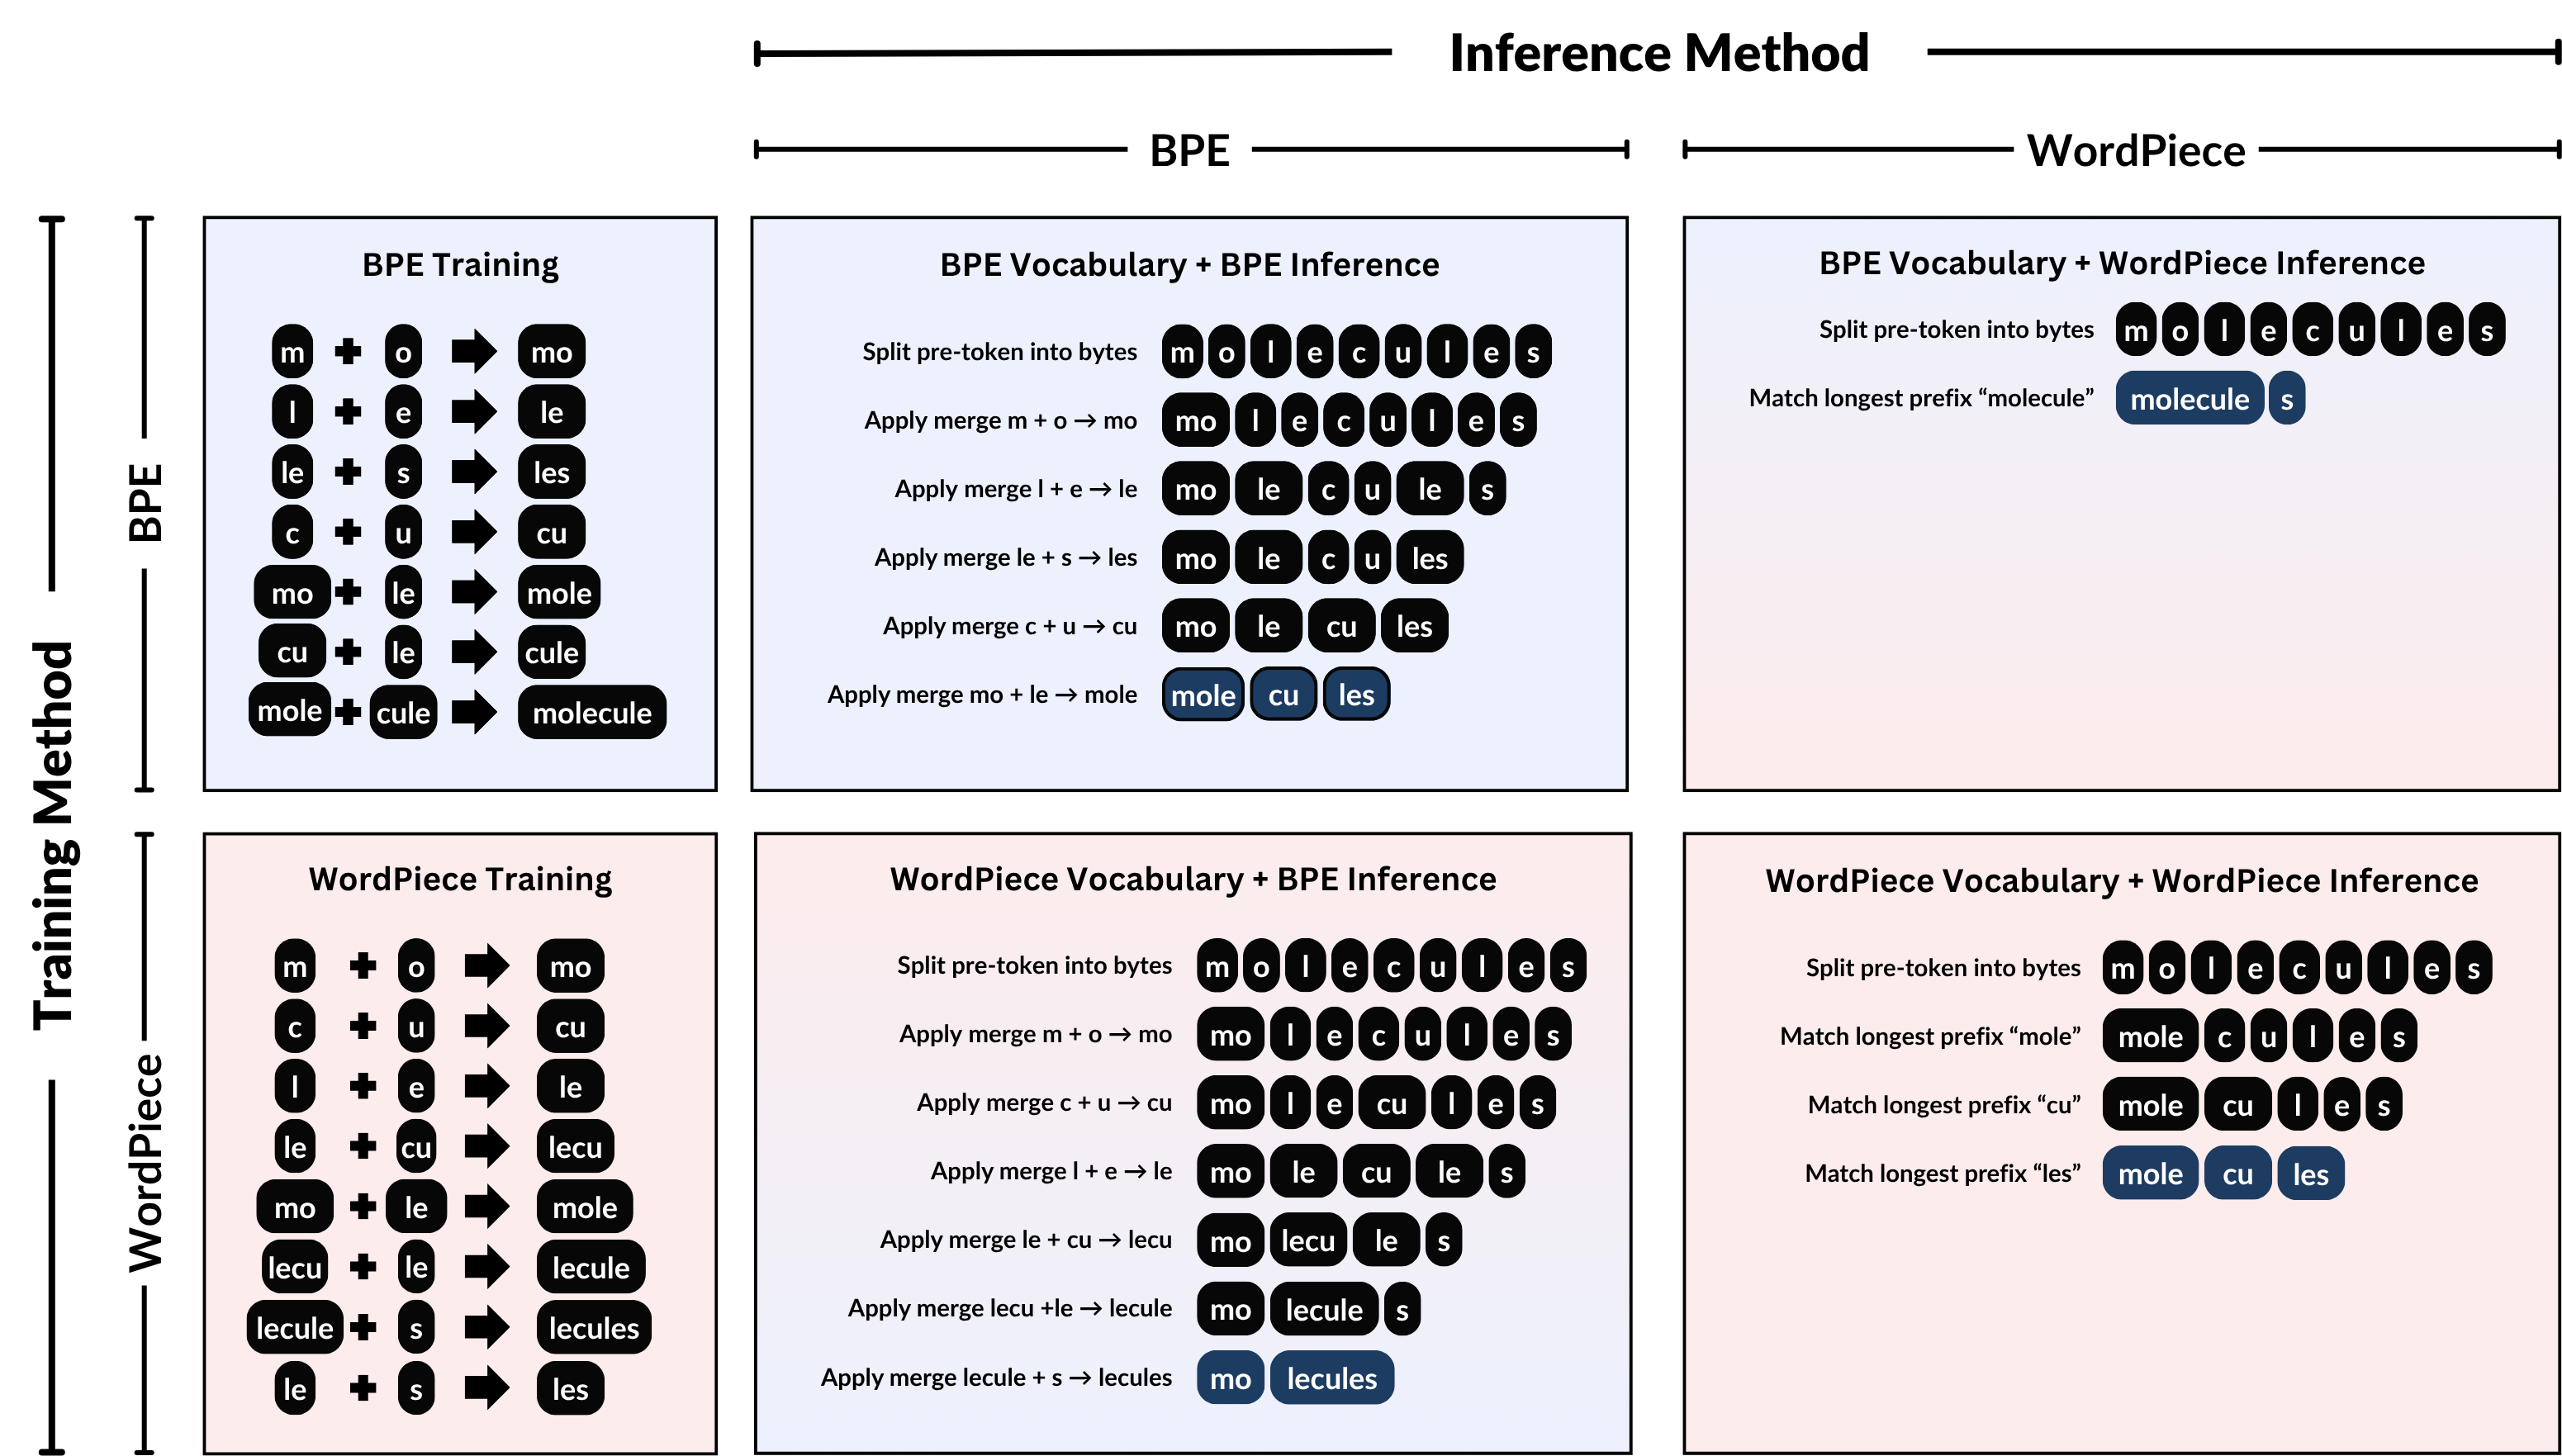
\includegraphics[width=0.99\linewidth]{12Background/tokenisers.png}
    \caption{Comparison of BPE and WordPiece training and inference procedures on the word \ex{molecule}. Merge operations are illustrative and not derived from real training data.}
    \label{fig:12-tokenisers}
\end{figure}

For a given vocabulary, BPE and WordPiece apply distinct tokenisation functions $\tok$ to segment pre-tokens into subword tokens. BPE operates via iterative merging: it begins by splitting pre-tokens into bytes, then greedily applies the merges learned during training. WordPiece uses a longest-prefix matching strategy: for a given pre-token, it recursively identifies and segments off the longest prefix found the vocabulary, repeating this process until the entire pre-token is segmented.

Tokenizer function strategies are also known as \defn{inference methods}. The training and inference methods for BPE and WordPiece are illustrated in \cref{fig:12-tokenisers}. Like their training procedures, both inference methods are greedy and do not necessarily yield the most compressive segmentation for a given vocabulary. For instance, both tokenisers segment \ex{molecules} into three tokens --- ${\ex{mole},\ex{cu},\ex{les}}$ --- even though more compressive segmentations are possible with their respective vocabularies. Because training and inference methods are independent, one can pair the inference method of one subword model with the training method of another, as explored by \citet{uzan-etal-2024-greed}. In \cref{fig:12-tokenisers}, these cross-model pairings yield more efficient segmentations comprising of just two tokens.
%\footnote{Note that this is a constructed example for illustrative purposes.} 

While BPE and WordPiece are widely used representative examples of subword tokenisation, many alternative methods have been proposed. For example, the UnigramLM objective operates in the other direction --- initially starting with a very large vocabulary (which could consist of all substrings, or could be learned using BPE), the method iteratively removes items that have the least effect on the loss given by a unigram language model \citep{kudo-2018-unigram}. These popular methods also have many alternatives and extensions, as described in the next section.
For a broader survey of subword tokenisation techniques in NLP, see \citet{mielke2021between}.
% REMOVE THE SURVEY?

\subsection{Limitations of subword-based representations}\label{sec:12-subwordlimitations}

While data-driven subword tokenisation algorithms offer practical advantages, a substantial body of research has highlighted their limitations and proposed various extensions, as outlined below.

\paragraph{Pre-tokenisation.} Some tokenisers, such as SentencePiece \citep{kudo-richardson-2018-sentencepiece}, avoid pre-tokenisation altogether by operating directly over raw characters or bytes. Supporting both BPE and UnigramLM, SentencePiece is especially useful in multilingual settings and for languages without explicit word boundaries. In contrast, most subword tokenisers rely on pre-tokenisers that split text at whitespace and often prefix tokens with a dedicated space character to mark word-initial positions. These conventions have increasingly been called into question. For instance, \citet{schmidt2025boundless} and \citet{liu2025superbpespacetravellanguage} propose \emph{superwords} by relaxing pre-tokenisation constraints, improving compression and promoting more uniform token distributions. Likewise, \citet{gow-smith-etal-2022-improving} argue against including spaces as token prefixes, showing that treating spaces as standalone tokens improves the segmentation of complex words without sacrificing downstream performance.

\paragraph{Morphological alignment.} Using data-driven methods like BPE can often result in subword units that overlap or misalign with morphemes. Many studies have theorised that morphological alignment is a desirable property for tokenisers to have, especially for machine translation systems that must handle morphologically-rich languages \citep{pan2020morphological}. Several extensions to popular subword algorithms have been proposed to improve morphological alignment, such as BPE-knockout \citep{bauwens-delobelle-2024-bpe} and MorphBPE \citep{asgari2025morphbpe}. Often, extensions are developed for specific languages, such as those proposed by \citet{kildeberg2025sm} for Dutch and \citet{nzeyimana-niyongabo-rubungo-2022-kinyabert} for Kinyarwanda. As a more general method, the SaGe tokeniser uses an objective $\obfn$ based on contextual similarity, rather than frequency, to select tokens during training, which was found to increase language modelling performance for both English and Turkish \citep{yehezkel2023incorporating}. 

\paragraph{Cognitive modelling.} LMs continue to be widely used in computational psycholinguistics to test theories that relate surprisal to human language processing \citep{shain2024}. However, subword tokens do not typically align with regions of interest, making it challenging to compute relevant probabilities. For instance, \citet{lesci2025causal} find that if a word is included in a tokeniser's vocabulary, the resulting probability can be up to 17 times higher than if the word is split into subwords and \citet{jumelet2025multiblimp10massivelymultilingual} find that this also has a significant effect on a multilingual linguistic benchmark. \citet{giulianelli-etal-2024-proper} argue that subword-based LMs should be marginalised into character-level models before the surprisal of substrings are computed to be used as psychometric predictors. Similarly, \citet{bunzeck2025subwordmodelsstruggleword} find that subword models struggle with word-level tasks. Separately, \citet{beinborn-pinter-2023-analyzing} analyse the cognitive plausibility of subword tokenisers according to whether the number of tokens produced for words correlates with human performance in a lexical decision task. Finally, \citet{fan-sun-2023-constructivist} argue for the necessity of a constructivist approach to tokenization, training an LSTM model on gold labelled data to tokenise text into morphemes, claiming that this enables the training of computational models that more closely align with language comprehension and acquisition. 

\paragraph{Multilingual modelling.} Besides morphological alignment, popular tokenisers have also been criticised for how they represent languages in multilingual settings. For instance, \citet{rust-etal-2021} compare the performance of multilingual tokenisers on monolingual tasks, finding that although balanced training data is useful, specialised monolingual tokenisers consistently improve downstream performance. \citet{limisiewicz-etal-2024-myte} note a different bias; that the character-to-byte conversion of byte-level BPE tokenisers results in significantly shorter sequences for Latin script languages, since letters are typically mapped to individual bytes. They propose MYTE as an improved character-to-byte scheme to more fairly model languages with diverse scripts. Finally, noting that subword tokenisation may not be appropriate for non-concatenative languages like Arabic, Hebrew and Malay, \citet{gazit2025splinteringnonconcatenativelanguagesbetter} introduce \emph{Splinter}, a pre-processing step which rearranges text to better represent non-concatenative morphologies.

\paragraph{Evaluation.} Evaluating subword tokenisers is difficult since comparing a suite of tokenisers would require pre-training language models from scratch using each, and the scaling laws mean that downstream effects may only not be apparent unless large models are used \citep{wei2022emergent}. Typically, studies address this by trying to find \emph{intrinsic} properties (e.g. properties that can be computed without a language model) that correlate with \emph{extrinsic} behaviour (performance of pre-trained language models), allowing later studies to use these metrics as a proxy. Many such measures have been proposed, the simplest of which are proxies for compression, such as fertility \citep{acs2019exploring}. \citet{zouhar-etal-2023-tokenization} hypothesise that the \renyi efficiency of tokenisers correlates with language modelling capabilities, whereas \citet{lotz2025beyond} hypothesise that tokenisers that produce more Zipf-like token distributions are preferable. Separately, \citet{beinborn-pinter-2023-analyzing} propose a `cognitive plausibility' score and several measures of morphological alignment have also been proposed \citep{gow-smith-etal-2022-improving, batsuren2024evaluating, arnett2025language}.

However, despite the number of criticisms and intrinsic properties discovered, it remains unclear what properties are desirable in a tokeniser. BPE, for instance, is argued to be effective since it compresses text into shorter sequences \citep{galle2019investigating}. However, a formal analysis of BPE reveals that compression is not the objective that BPE optimises for \citep{zouhar2023formal} and tokenisers that do directly optimise for compression lead to worse language modelling performance \citep{schmidt2024tokenization}. 

While individual intrinsic measures such as morphological alignment, cognitive plausibility or those that measure Zipfian distributions are hypothesised to be important for particular tasks, tokenisers that optimise for one often trade-off another \citep{uzan-etal-2024-greed, lotz2025beyond}. In general, just as the ``one size fits all'' paradigm for LLMs is not appropriate for all domains (as discussed in \cref{sec:12-domainspecific}), there is unlikely to be a subword tokeniser suitable for all purposes, and subwords themselves may not be the appropriate representation for certain domains. Instead, these limitations should encourage researchers to consider the input representation more carefully depending on the task and domain being modelled.

\subsection{Alternative input representations}\label{sec:12-alternative}

The limitations and extensions discussed in the previous section still primarily focused on subword-based representations. Below, alternative input representations that have been deployed in LMs are briefly surveyed.

\paragraph{Patching.} The quadratic cost of self-attention and the high per-position cost of large feed-forward networks have limited the ability of LLMs to model very long sequences. To address this, \citet{yu2023megabyte} introduce the concept of \defn{patching}. In this framework, byte embeddings are concatenated to form patches—units that roughly correspond to subword token, which are then processed by a global transformer. The resulting patch representations are decoded by a local transformer, which can even model raw audio. \citet{pagnoni2024byte} extend this idea to latent patches: instead of using fixed-length windows, the model segments variable-length patches in a latent space, with boundaries determined by the next-byte entropy estimated by a byte-level model. Overall, patching aims to improve the computational efficiency of language models beyond what subword tokenisation alone can achieve \citep{shao2025beyond}.

\paragraph{Character and byte-level.}
Despite the higher computational costs associated with character-level tokenisation, it has been actively explored as an alternative to subword units, motivated in part by the desire to build models that are more robust to noise and better capture morphological variation \citep{gupta2019character}. \citet{al-rfou_character-level_2019} show that sufficiently deep transformers can match the performance of subword- or word-level models, suggesting that the transformer architecture is largely agnostic to input granularity. \citet{libovicky-fraser-2020-towards} further demonstrate that this depth can be reduced by fine-tuning subword-level models and \citet{pinter2021learning} demonstrate how subword tokens can be augmented with character-level information. This line of work also includes byte-level models, such as ByT5 \citep{xue-2022-byt5}, which operate directly on raw bytes --- a natural choice when following the ``principle of modelling the smallest meaningful units in the data'' \citep{graves2013generating}. Finally, \citet{videau2025bytesideaslanguagemodeling} introduce a hierarchical auto-regressive architecture that reads bytes, pools them into words, then pools words into multi-word units at deeper stages, finding that this system can better handle character-level tasks compared to BPE while remaining computationally efficient. 
Character- and byte-level approaches are often described as \emph{token-free} \citep{clark-etal-2022-canine, xue-2022-byt5}, although \citet{mielke2021between} argue that this label is misleading: these models still rely on a fixed, predefined tokenisation scheme --- one that simply aligns with how data is conventionally stored on disk.

%https://aclanthology.org/P19-1491.pdf for varying between character and word-level in BPE

\paragraph{Representations beyond text.}

While most work in natural language processing focuses on text-based tasks, recent advances have extended large language model (LLM) architectures to the multimodal setting. These Multimodal Large Language Models (MLLMs) require input representations to handle these modalities. For joint image and text processing, the standard approach combines subword-based tokenisation for text with independently derived image tokens \citep{cui2024survey, team2024chameleon, liu2023visual}. Inspired by the robustness of human visual perception, some studies have explored using image-based representations even for purely textual tasks. For example, in the context of machine translation, \citet{mansimov-etal-2020-towards} investigate pixel-to-pixel translation models, and \citet{salesky-etal-2021-robust} render text as images. Both approaches demonstrate improved robustness to noise, though they typically underperform compared to models that operate directly on text.

In the speech domain, older speech-processing systems often relied on supervised acoustic models in combination with phoneme-level language models (see \cref{sec:12-ngrams}). In contrast, current state-of-the-art models learn directly from raw audio representations. Some approaches convert continuous speech into discrete units using self-supervised models such as Wav2Vec \citep{baevski2020wav2vec} or \myemph{HuBERT} \citep{hsu-2021-hubert}, and then apply standard language models to these sequences \citep{lakhotia2021generative}. Others, like Whisper, are trained end-to-end to map encoded audio directly to text \citep{radford2023robust}. Whereas speech-based representations are primarily used in multimodal or speech-focused settings, there have been efforts to integrate phonological units into pre-trained LLMs \citep{nguyen-etal-2025-spirit} or during pre-training \citep{bapna2021slam}. Typically, these models perform well on both modalities, but do not successfully learn better representations from exposure to multiple modalities --- an issue known as the transfer interference problem \citep{arivazhagan2019massively} --- and as a result, perform worse on text-based tasks than models solely trained using text-based representations. 

Finally, discrete phonemes provide an intermediate representation between raw audio and written text, as introduced in the next section. %Phonemic representations are compared against audio-based representations in \cref{sec:12-whynot}.

%CHAT: This thesis explores their potential as a linguistically meaningful alternative to audio-based representations, with a comparison presented in \cref{sec:12-whynot}.

\section{Phoneme-based input representation}\label{sec:12-phonemic}

Phoneme-based input representations consist of tokens representing individual phonemes. These tokens have a similar granularity to character-based representations --- indeed, in many languages there is a close correspondence between characters and phonemes, but other languages have much more opaque orthographies, like English. In contrast to character-based representations, phonemes are typically fed to a model in a sequence that does not contain punctuation, whitespace or other artefacts of written text. In particular, this means that words are not delimited by whitespace, as utterances are typically produced continuously, with no pauses between individual words.

%Despite phoneme-level language models having been used in early speech processing technology, there are few examples of phonemes being leveraged in modern auto-regressive architectures. Historically, the phoneme-based representation has been consistently used to study how children learn to segment words during language acquisition --- the word segmentation problem, as introduced in \cref{sec:12-wordseg}. 

This section first introduces how phoneme-based input representations are constructed in \cref{sec:12-implementphoneme}. Next, the word segmentation problem is introduced in \cref{sec:12-wordseg} --- an example of how phoneme-based representations have provided insights into human language acquisition, which also happens to have similarities to modern subword tokenisation methods. \Cref{sec:12-phonexperiment} presents other examples of the phonemic representation being used in phonological experimentation, where the use of LMs are providing unique insights about the distributional properties of language. Finally, \cref{sec:12-practicalphoneme} explores how modern architectures have benefited from the universality and cross-linguistic nature of phoneme-based representations to improve performance on downstream tasks.

Despite the practical and analytical benefits of phoneme-based input representations, their use in modern auto-regressive architectures have been largely unexplored. The language models used to study word segmentation predate transformers, the modern architectures used in phonological experimentation operate primarily at the word-level, and the models integrating phonemes to improve downstream performance are all auto-encoder architectures, which cannot easily generate text or provide next-phoneme predictions. Concluding this section, \cref{sec:12-phoneval} argues that there are many insights that can be gained from this research.

%And subword-level models struggle at word-level tasks. \citep{sims2025stochastokimprovingfinegrainedsubword,bunzeck2025subwordmodelsstruggleword}.

\subsection{Construction of phoneme-based input}\label{sec:12-implementphoneme}

Phoneme-based input representations are typically constructed from transcriptions of speech. Unlike written text, where languages have fixed orthographies, spoken language is transcribed using a variety of alphabets. These transcriptions can vary in the level of detail: broad \emph{phonemic} transcriptions consist of \defn{phonemes} --- the smallest contrastive units of sound in a language --- while narrow \emph{phonetic} transcriptions consist of \defn{phones}, the physical realisation of phonemes. A single phoneme may correspond to multiple allophones, depending on factors such as position within a word or surrounding context. In this thesis, the term \defn{phoneme} is used more broadly to refer to speech sounds, without specifically distinguishing abstract or concrete realisations. This usage aligns with the more general term \defn{segment}, which denotes a unit in a sequence of speech, as opposed to \emph{supra-segmental} features like stress and intonation. 

The most comprehensive and widely used system for transcribing speech is the International Phonetic Alphabet \citep[IPA][]{international1999handbook}, which provides a rich inventory of symbols for phonemes, along with diacritics for capturing finer phonetic detail. In addition to the IPA, other phonetic alphabets have been developed for specific linguistic contexts --- such as the Americanist Phonetic Notation for indigenous languages of the Americas \citep{lehmann2013historical}, and the Uralic Phonetic Alphabet for Uralic languages \citep{abondolo1998uralic}. Several ASCII-based alternatives, such as SAMPA \citep{wells1992standard} and the Kirschenbaum Phonetic Alphabet \citep{kirshenbaum2011ascii}, were designed for machine readability and digital use, mapping IPA symbols to standard keyboard characters. Since conversion tables exist between these systems, the specific choice of alphabet is often a matter of convenience rather than principle. Throughout this thesis, IPA is used as the primary transcription system.

Compared to the complexities of subword tokenisation, creating phoneme tokens from transcripts is relatively straightforward. However, depending on the transcription system, simple character-level tokenisation may be inadequate. For example, in the IPA, the affricate phoneme \textipa{tS} is represented by two Unicode characters; a character-level tokeniser would mistakenly split it into \textipa{t} and \textipa{S}, both of which are valid phonemes on their own. To avoid such ambiguity and simplify tokenisation, transcripts typically insert whitespace between phonemes. For example, the phrase ``molecules are unstable'' could be transcribed as \ex{\textipa{m A l I k u: l z A \*r 2 n s t eI b @ l}}. Thus, splitting on whitespace reliably produces accurate phoneme tokens. The difference between phoneme-level tokens and character-level tokens is illustrated in \cref{tab:12-granularity}.

The main challenge in constructing phoneme-based input representations therefore typically lies not in tokenisation, but in obtaining high-quality phonemic transcriptions. Unlike written text, which is abundantly available online, phonemic data remains relatively scarce. This limitation was recognised in earlier work using \ngram models for phoneme-level modelling, leading to the development of grapheme-to-phoneme (G2P) tools for creating phonemic datasets. \Cref{chapter:resources} provides a detailed review of these tools and existing phonemic datasets. Noting the limitations of these resources, it also introduces a new tool used to prepare a novel dataset for the experiments presented in this thesis.

\subsection{Word segmentation}\label{sec:12-wordseg}

Phoneme-based input representations are commonly used in the study of the \emph{word segmentation problem} --- how children learn to segment continuous speech into discrete words despite the absence of clear boundaries and a pre-existing lexicon. While adults can rely on their mental lexicon to segment novel utterances, children must bootstrap this ability, acquiring both segmentation skills and an initial lexicon by as early as six months of age \citep{Jusczyk1999infants}.

Experimental work on statistical learning has identified numerous cues that infants may leverage to segment speech \citep{Cutler1987, gleitman1988learning, Jusczyk1993stress, Saffran1996distributional, Jusczyk1999allophonic, Suomi1997}. Particularly influential were the findings of \citet{Saffran1996learning}, who demonstrated that 8-month-old infants use distributional information --- specifically, the fact that low conditional probability between adjacent syllables is often indicative of a word boundary. The principle that units within words are more predictable than units across word boundaries dates back to \citet{harris1955}.

These insights have motivated a variety of computational models that aim to demonstrate cognitively plausible segmentation strategies. Many models draw on a framework established by \citet{Brent1999}, who proposed a phoneme-level unigram language model for segmenting spontaneous child-directed speech. The input consisted of orthographic transcripts from \citet{bernstein1987phonology}, which Brent hand-transcribed into phonemes using a custom ASCII-based alphabet. Word boundaries were omitted, but utterance boundaries were preserved, consistent with evidence that children may use these cues to bootstrap lexical learning \citep{aslin1996models}. For example, the sentence ``you want to see the book'' was transcribed as ``yuwanttusiD6bUk''\footnote{Note that unlike IPA, this custom alphabet uses no more than one character per phoneme.}. This dataset of 9,790 utterances --- known as the BR corpus --- became a standard benchmark for segmentation models. Importantly, these models operate in an unsupervised setting, learning from the same input they are tasked with segmenting.

%Brent also established the typical metrics used to evaluate word segmentation performance (see \cref{sec:15-evaluation}) and phonemically transcribed 10,000 utterances from the Bernstein-Ratner \citeyear{bernstein1987phonology} corpus in CHILDES which continues to be used to evaluate segmentation models. 

Subsequent models introduced higher-order \ngram dependencies \citep{Venkataraman2001} and phonological constraints \citep{Blanchard2010}. Bayesian non-parametric approaches, such as those by \citet{Goldwater2009} and \citet{algayres_dp-parse_2022}, placed priors over word frequencies and phonological forms. Other models aggregated multiple statistical cues—such as different-length \ngrams and combined them through majority voting schemes \citep{ccoltekin2014explicit, Coltekin2017, goriely2023word}, with each cue producing a signal that peaks near likely word boundaries.

% Neural language models have also been leveraged for this task. For instance, in the foundational work of \citet{elman-1990-finding}, a simple recurrent network (SRN) is trained to predict letters in an unsegmented sequence. Analogously to the majority vote models above, Elman notes that the prediction-error increases at the onset of each new word, concluding that ``there is information in the signal that could serve as a cue to the boundaries of linguistic units which must be learned''. This principle was later leveraged by \citet{christiansen1998learning}, who used an SRN to segment speech represented with phonemes by using the probability of an \emph{utterance} boundary, rather than prediction-error, to place word boundaries.

Neural models have also been explored for segmentation. For example, \citet{christiansen1998learning} used the prediction of an utterance boundary from a simple recurrent network (SRN) to predict word boundaries. More generally, in a formative analysis of character-level RNNs, \citet{elman1990finding} observed that the prediction error could serve as a cue for lexical boundaries more broadly; boundaries around words, morphemes, but also frequent multi-word sequences, which children often treat as fixed lexical items \citep{macwhinney1978}. Neural models have also been used in a word segmentation task as part of the Zero Resource Speech challenge, which uses representations learned directly from audio, rather than phoneme-based representations, as discussed further in \cref{chapter:discussion}.

Strikingly, the core ideas behind these models closely mirror principles used in modern subword tokenisation. The \ngram-based segmentation models follow a similar objective as the UnigramLM algorithm \citep{kudo-2018-unigram}, and the multiple-cue methods and neural model prediction error methods closely resemble recent patching methods \citep{pagnoni2024byte}. Although this conceptual overlap has been noted in surveys \citep{mielke2021between}, segmentation models of phonemic transcriptions have yet to be explicitly leveraged to inspire new tokenisation algorithms, nor have they been revisited in the context of modern language model architectures.

%Discuss what phoneme-level segmentation reveals about inductive biases or learning difficulty

%Soon after word2vec, \citet{ma2016learning} presented a model that learned phoneme embeddings using the  a word segmentation task


\subsection{Phonological experimentation}\label{sec:12-phonexperiment}

% Add \citep{prince-1997-optimality}?

Besides word segmentation, phoneme-based input representations have been used more broadly to study human language processing and the distributional patterns of speech. Building on ideas from the theoretical COHORT model of \citet{MARSLENWILSON1978}, foundational models incorporating phonemic input include the TRACE model of speech perception \citep{mcclelland1986trace}, the distributed model of lexical access by \citet{seidenberg1989distributed}, the SHORTLIST model \citep{norris1994shortlist}, and the dual-route cascaded (DRC) model of visual word recognition \citep{coltheart2001drc}. These models relied on phoneme-based input to simulate phonological aspects of language comprehension, capturing how listeners incrementally interpret spoken language over time. Furthermore, the architectures employed in these models --- particularly TRACE and the \citet{seidenberg1989distributed} model --- were closely aligned with early developments in connectionist and neural network approaches, marking a historical convergence between cognitive theories of speech perception and the computational modelling of linguistic representations.

Phoneme-based representations remain valuable tools for phonological and cognitive experimentation in the era of modern language models. For example, \citet{kirov-2018-recurrent} revisit the classic connectionist model of \citet{Rumelhart1986}, which learns the past tense of English verbs from phonemic input. While this earlier model was famously criticised by \citet{pinker_language_1988}, who argued that neural networks could not account for rule-based generalisation in past tense formation, \citet{kirov-2018-recurrent} show that a modern LSTM encoder-decoder architecture can obviate these criticism, successfully generalising to novel verb forms. In a separate line of work, \citet{pimentel2020phonotactic} employ phoneme-level LSTM language models to quantify the phonotactic complexity of 106 languages. They find a robust inverse correlation between model-assigned bits-per-phoneme and average word length, suggesting an efficiency trade-off between phonotactic permissiveness and lexical economy. Notably, both of these studies model phoneme sequences at the level of word types rather than full utterances. Phoneme-level models have also been used in cognitive neuroscience: \citet{donhauser2020two}, for instance, compare predictions from word-level and phoneme-level LSTM models to human brain responses, exploring how hierarchical predictions unfold during real-time speech processing.%\zeb{insert \citet{lavechin}}

In word segmentation research and the studies discussed above, phoneme-based representations are employed because the underlying theories assume that phonemes are the fundamental units over which learning and processing occurs. Additionally, when studying acquisition, care is taken to use transcripts of child-directed speech as input. While it remains debated whether infants possess phonetic categories prior to acquiring a lexicon \citep[e.g.][]{feldman_infants_2021}, or how phonemes are accessed during real-time language processing \citep[e.g.][]{mcmurray_myth_2022}, the broader methodological point holds: for phonological experimentation, it is crucial to adopt a representation aligned with the theoretical assumptions being tested.

An apparent counterexample is PhonologyBench \citep{suvarna-etal-2024-phonologybench}, a benchmark that uses natural language prompts to probe phonological knowledge in English LLMs. This approach aligns more with LLM interpretability than with genuine phonological inquiry. As argued in \cref{sec:12-domainspecific}, LLM performance on such benchmarks is unlikely to yield insights into human language acquisition or processing. Moreover, by relying on prompting, the benchmark treats phonology as an emergent ability tested through metalinguistic judgment --- an evaluation strategy which \citet{hu2023prompting} argues is less informative than using quantities directly derived from a model's representations. 

\subsection{Practical applications of phoneme LMs}\label{sec:12-practicalphoneme}

Phoneme-based input representations remain relatively uncommon in practical LM training. This is partly due to the success of recent end-to-end models that operate directly on audio, as discussed in \cref{sec:12-alternative}. However, such models are extremely data-hungry \citep{li2022recent}, making them impractical for the 7000+ human languages which are considered under-resourced \citep{scharenborg2020speech}. In this context, phoneme-level models continue to play an important role in speech-focused applications.

Several studies have explored phoneme-level \bert-style architectures for specific speech tasks. For instance, \citet{jia2021png},  \citet{zhang2022mixed} and \citet{li-2023-phoneme-level-bert} train phoneme-level models to improve phoneme representations for text-to-speech, combining phonemic and graphemic input and output in various configurations. Similarly, \citet{sundararaman-2021-phonemebert} propose a \bert model that jointly encodes aligned phoneme and grapheme sequences to enhance ASR, particularly in noisy or out-of-domain settings.

Building on the cross-linguistic nature of phonemes, \citet{li2020universal} demonstrate that combining language-independent phones with language-specific phonemes benefits low-resource ASR. In related work, \citet{feng-2023-language-universal-phonetic} introduce phoneme-informed supervision into \myemph{HuBERT} to boost ASR performance in low-resource scenarios.

There are few examples of phoneme-based representations being leveraged in LMs outside of speech tasks. Noting this, \citet{gale-etal-2023-bort} present BORT (Beyond Orthographically Restricted Transformers), a general-purpose model that learns jointly from orthographic and phonemic inputs, and show its effectiveness on pronunciation tasks. Finally, \citet{leong-2022-phone} argue that phoneme-based input representations can be particularly effective for low-resource modelling, especially for languages where there is little or no written data, by converting audio and text input to phonemes. They utilise phone recognition technology and G2P to map both audio and text to IPA to train phoneme-level \bert-style models, demonstrating that this flexible pre-training method improves Named Entity Recognition (NER) performance for Swahili and Kinyarwanda. 

% Besides being primarily aimed at speech-focused applications, these models are also auto-encoder architectures, trained with the MLM objective, so cannot easily be leveraged as language models that provide next-phoneme predictions. It seems that beyond phonological experimentation, the use of phoneme-based representations in auto-regressive architectures has been largely unexplored.

While these phoneme-based \bert-style models have shown promise in speech-related tasks, they are trained using the MLM objective within an auto-encoder framework. As a result, they are not naturally suited for next-phoneme prediction or standard language modelling tasks. Beyond targeted phonological experiments, the use of phoneme-based representations in auto-regressive architectures remains largely under-explored.

\subsection{The role of phoneme-based input}\label{sec:12-phoneval}

The literature reviewed above indicates that phoneme-based representations in NLP are currently used primarily for phonological experimentation, though they do offer practical advantages in speech-based applications. Their language-agnostic properties support cross-lingual transfer, and their relatively low data requirements make them especially suitable for under-resourced languages --- unlike data-intensive end-to-end models.

While phoneme-based inputs have been used in auto-encoder models for speech tasks and in auto-regressive models for specific phonological experiments, their broader potential as input representations for LMs remains largely under-explored. A central hypothesis of this thesis is that contrasting phoneme-based inputs with standard subword-based inputs can serve as a diagnostic tool for probing how LMs learn linguistic structure. Given that most prior phonological work with LMs has focused on word-level tasks, this thesis also explores the insights that can be gained from utterance-level language modelling with transformer architectures. Moreover, connections between word segmentation and modern subword tokenisation suggest the possibility of developing new, linguistically informed tokenisation methods.

Testing these hypotheses requires a pre-training and evaluation framework that can meaningfully contrast phoneme-based models with standard LMs, while remaining grounded in the theoretical assumptions of prior phonological research. This includes using phoneme-level transcripts to study distributed phonology, and child-directed speech to investigate early language acquisition. The next section outlines this framework.

% Takeaways from above:
% - phoneme LMs are primarily used for phonological evaluation, but so far this has mostly involved models that train on individual words, rather than running text. phonemes are a more principled representation for these studies, where it is important to use developmentally-plausible data.
% - phonemes are practically useful in speech-based applications, primarily for low-resource settings (where end-to-end is impractical) and for cross-lingual transfer, due to a shared representation between languages.
% - the broad capabilities of LMs trained with phonemes has not been studied, nor has the phoneme-based representation been thoroughly compared against subword-based representations


% This thesis argues integrating phoneme-based input into auto-regressive LMs:
% - can continue to provide analytical insights into phonological structure across languages and the distributional role of phonemes
% - can act as a diagnostic tool for understanding how language models learn linguistic structure by contrasting to subword-based representations, e.g. do LMs need word boundaries, or are they learned implicitly --- additionally drawing from word segmentation could provide insights into subword tokenisation methods

% To gain insights across these two, we need a good framework for training and evaluating phoneme LMs.  it is important to train phoneme LMs in a manner that can be contrasted with typical LM pre-training (for (2)) while also training on data that is developmentally plausible (for (1)). The framework of developmentally-plausible pre-training satisfies both, as introduced in the next section.


% One method for testing phonology is to use minimal pairs of words and pseudowords as a lexical decision task. One benchmark that uses this approach is BabySLM \citep{lavechin}, which provides a lexical decision metric for phoneme LMs or speech LMs (which learn directly from audio) using a vocabulary based on child-directed speech. \citet{bunzeck-etal-2025-small} use a similar approach in order to compare grapheme LMs to phoneme LMs. They also use two probing tasks to examine the representations of sentences; age prediction and rhyme prediction. %These studies only test English models, in part due to the lack of phoneme LMs in other languages, but also due to a lack of resources for constructing phonological tasks. For example, they both use \texttt{wuggy} \citep{keuleers2010wuggy} to generate pseudowords, which only supports three languages for phonetic pseudoword generation.

% %Very few methods for measuring phonological evaluation of LLMs. PhonologyBench is one example but is based on prompting for very large language models trained on orthographic text, limiting analysis of representations learned for individual phonemes. BabySLM provides a lexical decision task, more closely relating language models to psycholinguistic studies of human preference. \citet{bunzeck-etal-2025-small} use a similar test, also exploring rhyme prediction and age prediction as phonological tasks. These studies all only explore English phonology due in part to the lack of phonemic data in other language \citep{goriely2023word} as well as a lack of resources for constructing phonological tasks. For example, BabySLM uses Wuggy to generate pseudowords but Wuggy only supports three languages for phonetic pseudoword generation.


% These benchmarks also only test English models, in part due to the lack of phoneme LMs in other languages, but also due to a lack of resources for constructing phonological tasks. For example, pseudowords are typically generated using \texttt{wuggy} \citep{keuleers2010wuggy}, which only supports three languages for phonetic pseudoword generation. An example of language-independent evaluation of phoneme LMs is the phonetic feature probe used in \citet{goriely2025}, which only requires feature vectors for each IPA symbol. The word segmentation task requires no language-specific data, only utterances labelled with word boundaries. 

% % Compared to models trained on orthographic text or raw audio, few studies training with phonemes. Models based on BERT have shown that training with phonemes can be useful for downstream tasks. In comparison studies, grapheme models slightly outperform phoneme models \citep{nguyen-2022-word-boundaries, bunzeck2024graphemes} but this could be attributed to preprocessing differences, punctuation and the fact that typical LLM architectures have been optimized for written text \citep{goriely2024babble}. As with phonological benchmarks, few phoneme LMs exist for languages other than English. Here, we release phoneme LMs trained on the 31 languages in \ipachildes...


% \subsection{Why not use audio-based representations?}\label{sec:12-whynot}

% - discuss phoneme vs audio

% - mention that there is work in developmentally plausible settings, maybe forward that to the next?

%CHAT: In addition to orthographic and phoneme-based inputs, recent advances have produced language models operating directly on audio signals. Models such as wav2vec 2.0 and HuBERT learn speech representations end-to-end from raw waveforms, capturing acoustic and phonetic features implicitly. While these models excel in speech recognition and generation tasks, they require vast speech corpora and computational resources. Phoneme-based input representations offer a complementary approach, providing a linguistically interpretable symbolic abstraction that facilitates detailed phonological analysis and modelling with relatively modest data and compute. This thesis focuses on phoneme-level representations to leverage these advantages, while acknowledging the ongoing importance of audio-based models.
%This is revisited in discussion....

% CHAT: While some studies evaluate the phonological competence of large language models, these models are typically trained on orthographic input, creating a potential mismatch between the representational format and the linguistic phenomena being tested. Phoneme-based input representations offer a more direct mapping to the phonological domain and may yield models whose inductive biases better align with phonological generalisation. However, the use of such representations remains relatively rare, in part due to resource limitations — an issue addressed in Chapter [X].

% \Zeb{Combine cross-linguistic work here with phonological evaluation?}

% \Zeb{Some statement here about potential of phoneme tokenisation and the fact that alternative input representations are largely under-studied in NLP, due to the convenience of the default one. Maybe here go into the historical use of the input representation and that it has been vastly understudied. }

% \Zeb{Formal definition of what I mean by the phonemic input representation. This is where the three transformations are described. Similar to character-level. Maybe here worth going more into detail with character-level models and tabula rasa model.}

% % One reason could be a lack of resources, which is the topic of \cref{chapter:resources}. A benefit of exploring alternative input representations is to ablate the effect of each of the features of the default representation, as explored in \cref{chapter:modelling}. The cognitive aspect... \cref{chapter:phonology}... and could improve tokenisation methods... \cref{chapter:infotokenization}.

\section{Developmentally-plausible pre-training}\label{sec:12-plausiblepretraining}

% \Zeb{Idea that ``simulations must closely emulate real-life situations by training on developmentally plausible corpora'' in order to gain insights both about what language models can learn, and improve understanding about how infants learn language. Clearly could be valuable insights for phonology in this area.}

% \Zeb{BabyLM framework is appropriate for two reasons. Firstly, the scale: it's appopriate for academic budgets, phoneme models can be useful for low-resource, and phoneme data is too limited for larger scale models (see next chapter). Secondly, the developmental/analytical angle. These models have been branded as useful for cognitive research due to the developmental plausibility. Phoneme representation so far has mostly been used for analytical purposes, so using develpmentally plausible framework is logical - and using the phoneme representation provide an additional aspect of plausibility beyond written text and exploration is worthwhile.}

% \Zeb{Later, BabyLM challenge created a framework for training and evaluting such models. Still motivated by developmentally plausible data, but still using default input representation. Findings more about architectures for low-data than specifically for insights into human learning. This framework provides a good way of testing this size model.}

In recent years, there has been growing interest in pre-training smaller language models on developmentally plausible corpora, as introduced in \cref{sec:12-domainspecific}. By training models in settings that more closely emulate real-life language exposure, this line of research aims to illuminate both the capabilities of language models and the mechanisms underlying human language acquisition. A central initiative in this area is the BabyLM challenge, which coined the term \defn{BabyLM} to refer to language models trained on developmentally plausible data --- a convention adopted throughout this thesis.

One key goal of the BabyLM challenge is to establish a framework for pre-training research that remains accessible within academic budgets. As shown in \cref{fig:12-scales}, the training data is small compared to typical large-scale language model pipelines, yet the evaluation protocol includes benchmarks typically used to evaluate language models. Specifically, BLiMP assesses grammatical generalisations using minimal pairs, while GLUE evaluates downstream language understanding tasks through fine-tuning. The underlying assumption is that insights from small-scale models will extrapolate to larger scales, in line with established scaling laws \citep{kaplan2020scaling}. This framework therefore provides a useful setting for technically comparing the effect of pre-training with phoneme-based representations compared to subword-based representations.

A second aim of the BabyLM challenge is to shed light on the learnability of language by human infants. Here, the hypothesis is that language models trained on data that mirrors the scale and structure of early linguistic input can yield insights into human language development. However, research with this focus often relies on alternative corpora --- particularly transcripts from the Child Language Data Exchange System (CHILDES), an open-access repository of child-centred data. CHILDES is also commonly used in studies of word segmentation (\cref{sec:12-wordseg}) and phonological learning (\cref{sec:12-phonexperiment}) --- making it suitable for the phonological experiments conducted in this thesis.

The degree to which BabyLMs can inform theories of human language acquisition remains contested \citep{dupoux-2018-cognitive,baroni-2022-proper,warstadt-2022-artificial,beinborn2024cognitive,wilcox2025bigger,salhancopil2025}. Central to this debate is the importance of realism: to approximate human learning, it has been argued that the data and representational format must align with what infants actually encounter. While the BabyLM corpus is designed to be developmentally plausible, its reliance on subword units derived from text departs from infants' auditory experience. Phoneme-based representations, though still an abstraction, arguably better reflect the structure of spoken language and have been largely considered to be a sufficiently realistic representation in past word segmentation studies. More recent work, however, shows that it is feasible to train BabyLMs directly on audio. For instance, \citet{lavechin} introduce the BabySLM benchmark to compare models trained on audio, phonemes, and text, finding that phoneme- and text-based training still outperform direct audio training. % insert more here?

%Instead, LMs trained on developmentally-plausible corpora are used to study the distributional properties of language --- with grammatical capabilities of the models used to argue for the learnability of these rules from distributional properties, not that LM training mimics human learning mechanisms. 

Accordingly, the BabyLMs developed in this thesis are not intended as realistic simulations of child language acquisition. Instead, they are used as diagnostic tools to explore the distributional properties of speech across languages and to probe the phonological representations learned during training. Although \cref{chapter:modelling} includes a word segmentation task --- historically used to propose cognitively plausible mechanisms of early language learning --- the results are primarily interpreted according to model behaviour and distributional phonology. While findings on this task may also contribute to statistical learning theories, they must be weighed against the limitations of phoneme-based training. These limitations are further explored in \cref{chapter:discussion}, which also considers the broader question of whether phoneme-based BabyLMs can inform linguistic theory in light of recent advances in audio-based learning.

Note also that besides BabySLM, the datasets and evaluation metrics presented here are orthographic.\footnote{CHILDES is linked to TalkBank, which contains phonemic transcripts, but these are predominantly child-produced speech, limiting phonological experimentation using adult speech.} Using these to explore phoneme-based representations requires grapheme-to-phoneme conversion, as presented in \cref{chapter:resources}. 

The remainder of this section introduces the core resources and benchmarks used in this thesis. \Cref{sec:12-datasets} describes the BabyLM dataset and CHILDES, the two primary training corpora. \Cref{sec:12-evaluation} presents the evaluation benchmarks --- BLiMP, GLUE, and BabySLM --- used to investigate the effects of phoneme-based pre-training.



\subsection{Datasets}\label{sec:12-datasets}

The datasets used to train LMs in this thesis differ from typical pre-training datasets not only in scale, but also in domain. Samples from the BabyLM dataset and CHILDES are shown in \cref{tab:12-datasetexamples} in contrast to a sample from FineWeb-Edu\footnote{\href{https://huggingface.co/datasets/HuggingFaceFW/fineweb-edu}{\myemph{huggingface.co/datasets/HuggingFaceFW/fineweb-edu}}.} --- a 15T-token pre-training dataset consisting of web-scraped educational text \citep{penedo2024finewebdatasetsdecantingweb}. Below, the BabyLM dataset and CHILDES are described.

\begin{table}[t]
    \centering
    \footnotesize
    \begin{tabular}{p{0.85\textwidth}}
        \toprule
        \textbf{FineWebEdu} \\
        \midrule
        \texttt{Previous abstract Next abstract} \\
        \texttt{Session 40 - The Interstellar Medium.} \\
        \texttt{Display session, Tuesday, June 09} \\
        \texttt{Gamma Ray Burst (GRB) explosions can make kpc-size shells and holes in the interstellar media (ISM) of spiral galaxies if much of the energy heats the local gas to above 10\^{}7 K. Disk blowout is probably the major cause for energy loss in this case, but the momentum acquired during the pressurized} \\
        \midrule
        \textbf{BabyLM dataset} \\
        \midrule
        \texttt{Now if we think of W U as being er, the expected value of the urban wage, and that equals the probability of getting a job, multiplied by the actual urban wages, alright then this probability of getting a job is going to be important as well.} \\
        \midrule
        \textbf{CHILDES} \\
        \midrule
        \texttt{just like your book at home.} \\
        \texttt{see.} \\
        \texttt{there's a face with glasses.} \\
        \texttt{ahhah.} \\
        \texttt{look there's pooh bear.} \\
        \bottomrule   
    \end{tabular}
    \caption{Comparative examples from three datasets: FineWebEdu, BabyLM and CHILDES.}
    \label{tab:12-datasetexamples}
\end{table}



\subsubsection{The BabyLM dataset}\label{sec:12-babylmdataset}

The BabyLM dataset consists of data from pre-existing datasets, curated to reach a target of 100M words. These sources are chosen to reflect data that could plausibly be encountered by language-learning children, and so there is a high proportion of data from child-directed sources and spoken sources. The dataset was adjusted between the first and second edition of the challenge; this thesis uses the second version. 

\begin{table}[t]
    \centering
    \footnotesize
    \begin{tabular}{llr}
        \toprule
        \textbf{Dataset} & \textbf{Description} & \textbf{\# Words} \\
        \midrule
        CHILDES \citep{macwhinney1985child} & Child-directed speech & 29M \\
        British National Corpus \citep[BNC,][]{bnc2007} & Dialogue & 8M \\
        Project Gutenberg \citep{gerlach2018standardizedprojectgutenbergcorpus} & Children's stories & 26M \\
        Open Subtitles \citep{lison-tiedemann-2016-opensubtitles2016} & Film subtitles & 20M \\
        Simple English Wikipedia\footnotemark & Written simple English & 15M \\
        Switchboard Dialogue Act Corpus \citep{stolcke-etal-2000-dialogue} & Dialogue & 1M \\
        \bottomrule      
    \end{tabular}
    \caption{The datasets included in the BabyLM dataset, where \textbf{\# Words} specifies the estimated number of words used from each source.}
    \label{tab:12-babylm}
\end{table}

The data sources used to construct the BabyLM dataset are reported in \cref{tab:12-babylm}. A range of sources are used to reach the 100M word target, with 70\% of the data consisting of child-directed sources and 58\% of the data consisting of speech data. The most developmentally-plausible is CHILDES, which is both child-directed and speech --- as described in the next section --- but does not contain enough English transcript data to reach the 100M word target. Other sources like Project Gutenberg and Simple English Wikipedia are chosen to mimic simplified language, but as written sources do not contain pauses, interruptions or other artefacts of spoken language. On the other hand, Open Subtitles contains transcripts from films, but many of these films are scripted, and so again may not mimic naturalistic speech. The BabyLM sample shown in \cref{tab:12-datasetexamples} is from BNC --- as a transcript of naturalistic dialogue, hesitations and run-on sentences are more typical, but the semantic content is adult-directed.
\footnotetext{\href{https://dumps.wikimedia.org/simplewiki/}{https://dumps.wikimedia.org/simplewiki/}}

Models trained on the BabyLM dataset have led to the development of new architectures, notably \myemph{ELC-BERT} \citep{georges-gabriel-charpentier-samuel-2023-layers} and \myemph{GPT-BERT} \citet{charpentier2024gpt} --- two of the winning entries of past BabyLM challenges. Although the data comes from a variety of sources, this has supported data-driven experiments, such as the role of variation sets \citep{haga-etal-2024-babylm}, the effect of diverse data \citep{yam-paek-2024-baby} and curriculum learning strategies \citep[e.g.][]{debenedetto-2023-byte, nguyen-etal-2024-automatic, capone-etal-2024-concretegpt}.

Curriculum learning in particular has been thoroughly explored --- for example, in prior work submitted to the  first BabyLM challenge, my co-authors and I found that cognitively-driven curriculum-learning procedures largely did not have a significant effect on BLiMP and GLUE \citep{martinez-etal-2023-climb}. This seems to counter \citet{huebner-etal-2021-babyberta} --- whose finding that training BabyLMs on child-directed speech before Wikipedia increased grammatical performance likely inspired the partitioning of the BabyLM dataset --- although recent work has challenged this study, finding that adjusting for frequency effects in evaluation nullifies the advantage that this curriculum provided \citep{padovani2025child}. Although the best-performing models in past BabyLM challenges have primarily won due to innovative architectures, rather than methods that leverage the data distribution, the dataset is still a useful tool for comparing against other LMs of this size within the academic community.

% KidLM, chat-gpt generated dataset?

Another limitation of the BabyLM dataset is that is only contains English data. A similar dataset consisting of a variety of sources has been developed in German \citep{bunzeck2025constructiondistributionsshapeformal}, and future instances of the BabyLM challenge will include a multilingual track, but otherwise, BabyLMs trained in other language predominantly rely on data from CHILDES, as described in the next section. 

\subsubsection{The CHILDES database}\label{sec:12-childes}

The Child Language Data Exchange System (CHILDES) is a repository of child-centred data originally developed with the aim of preserving and standardising data used for child language development research \citep{macwhinney1985child}. The project later grew into TalkBank, which contains over 1.4TB of transcript data and 5TB of associated media data across several ``banks'' \citep{macwhinney_understanding_2019}. Each bank focuses on a different area of human communication, with a general focus on spoken communication, with the CHILDES banks now containing child-caregiver interactions in over 40 different languages thanks to the efforts of hundreds of contributors over the last 40 years. 

CHILDES is an extremely valuable resource for research on child language development and has led to many thousands of published articles since its release. Due to the commitment to open-data sharing, the influence of these resources has also extended to other fields of research. For instance, in a recent assessment on the impact of the TalkBank project, \citet{bernstein_ratner_augmenting_2024} noted that a corpus she had contributed to CHILDES --- originally collected to study the acoustic features of child-directed speech \citep{Ratner_1984}\footnote{Note that this is the same corpus that was phonemically transcribed by \citet{Brent1999} to create the BR Corpus, used in many of the word segmentation studies discussed in \cref{sec:12-wordseg}.} --- was still leading to new insights forty years later:
\begin{quote}
The corpus has been further used to test models of unsupervised induction of grammar in machine language learning \citep{glushchenko_programmatic_2019}, a prospect not remotely envisioned during the original study, when data were collected on reel-to-reel analog tapes, and acoustically analyzed using a dedicated mainframe computer that had to be booted with punched paper tape.
\end{quote}

Besides contributing to a portion of the BabyLM dataset, CHILDES has also been used elsewhere to explore BabyLM pre-training and what representations can be learned from child-directed speech. For instance, \citet{huebner_structured_2018} explored whether SRNs and LSTMs learn hierarchical representations when trained on data from CHILDES. \citet{yedetore-etal-2023-poor} later used LSTMs and transformer-based LMs, finding that models learn incorrect linear rules, rather than human-like generalisations. Additionally, \citet{huebner2021using} use the age information in CHILDES to create AO-CHILDES, used in the curriculum-learning experiments of \citet{huebner-etal-2021-babyberta}.

CHILDES has also supported cross-lingual work in this area. For instance, \citet{capone2024babies},\citet{shen2024bambino} and \citet{suozzi2025bambidevelopingbabylanguage} train Italian monolingual and bilingual BabyLMs using CHILDES, \citet{bunzeck2025constructiondistributionsshapeformal} train German BabyLMs, \citet{yadavalli2023slabert} use data from five language in CHILDES to explore second language acquisition theories and \citet{salhan-etal-2024-less} use age-ordered data from four languages in CHILDES to explore fine-grained curricula inspired by language acquisition. CHILDES is therefore a useful dataset for exploring cross-lingual phoneme-based BabyLMs both for architectural research and phonological experimentation.  

% For researchers seeking developmentally-plausible corpora to use as pre-training data for language models, CHILDES is a natural fit. For instance, BabyBERTa was pre-trained on the AO-CHILDES corpus (Age-Ordered CHILDES, \citep{huebner2021using}). AO-CHILDES contains approximately 5M words from the North American English sections of CHILDES. Specifically, it contains all utterances involving children aged 0 to 6, sorted by child age, with non-adult speech removed (thus simulating the theoretical input received by a child). In their study, \citet{huebner-etal-2021-babyberta} were interested in the outcome of pre-training BabyBERTa on AO-CHILDES compared to Wikipedia (which was considered a more representative dataset for NLP at the time). Using a linguistic benchmark based on BLiMP (see \cref{sec:12-blimp} below), they found that BabyBERTa achieved a higher accuracy when trained on AO-CHILDES, that the choice of corpora had an effect across the pre-training corpus and that ordering multiple corpora by grammatical complexity could `scaffold' learning. These findings validated the importance of using developmentally-plausible corpora for BabyLM research and the scaffolding results were a precursor of many of the curriculum learning approaches taken in the first edition of the BabyLM challenge \addcites.

\subsection{Evaluation metrics}\label{sec:12-evaluation}

Below are a description of the main benchmarks used to evaluate BabyLMs in this thesis. These are also illustrated in \cref{fig:12-evaluation}.

\begin{figure}[t]
    \centering
    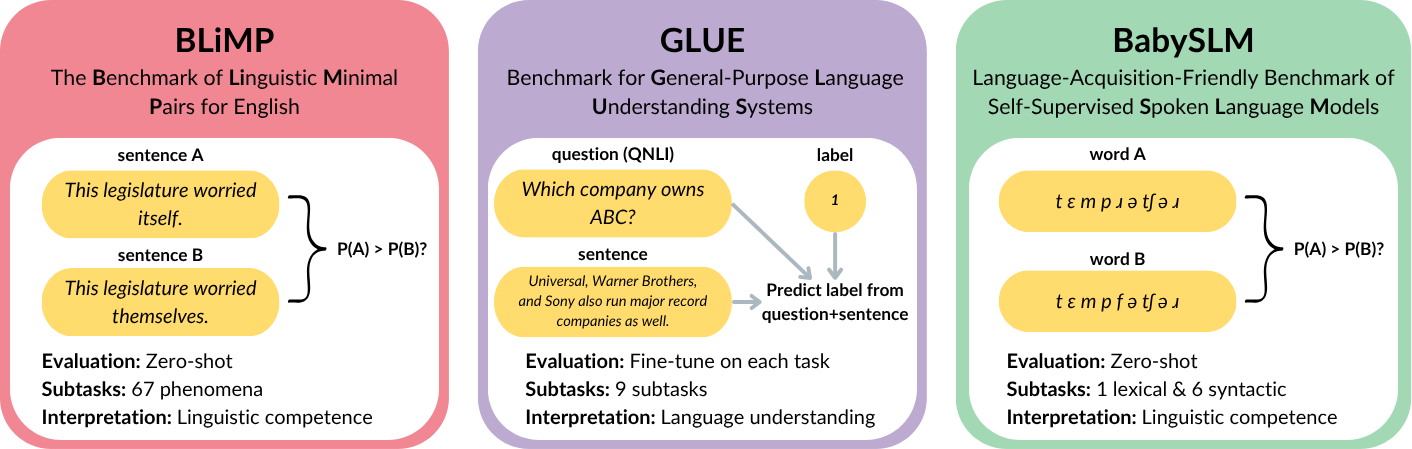
\includegraphics[width=0.99\linewidth]{12Background/evaluation.png}
    \caption{A summary of BLiMP, GLUE and BabySLM, with example test instances.}
    \label{fig:12-evaluation}
\end{figure}

\subsubsection{BLiMP}\label{sec:12-blimp}

The Benchmark of Linguistic Minimal Pairs \citep[BLiMP][]{warstadt-2020-blimp} provides a metric for linguistic competence across 67 subtasks, each representing a different linguistic phenomenon covering syntax, morphology and semantics. Each subtask contains 1000 pairs of grammatical and ungrammatical sentences that differ only with respect to the specific linguistic characteristic being tested. Language models are tasked with assigning a higher likelihood to the grammatical sentence than the ungrammatical sentence. The grammatical generalisation capabilities of a language model are often summarised by averaging the accuracies achieved across the subtasks. While random guessing scores 50.0, state-of-the-art models have achieved scores of 87.0 when trained on large datasets, and models trained on the BabyLM dataset have achieved scores up to 86.1 \citep{hu-etal-2024-findings}. 

BLiMP only tests for grammatical generalisations in English, but later minimal pair benchmarks have targeted other languages. These include JBLiMP \citep{someya-oseki-2023-jblimp} for Japanese, CLiMP \citep{xiang-etal-2021-climp} and SLING \citep{song-etal-2022-sling} for Chinese, and CLAMS \citep{mueller-etal-2020-cross}, which tests for subject-verb agreement in English, French, German, Hebrew and Russian. Most recently, MultiBLiMP assembled a benchmark of minimal pairs covering 6 phenomena in 101 languages \citep{jumelet2025multiblimp10massivelymultilingual} --- used to evaluate models ranging from huge multilingual LLMs (such as Llama-3) to small monolingual LMs (such as the Goldfish models).% INCLUDE THIS? It was released shortly before the submission of this thesis, after the experimental work was completed, but could be leveraged in future work.

BLiMP provides a useful benchmark for evaluating the linguistic competence of BabyLMs trained with a phoneme-based input representation. The BabyLM challenge also introduced 5 additional BLiMP tasks called BLiMP Supplement --- which focus on dialogue and questions, linguistic abilities not included in BLiMP \citep{warstadt-2023-babylm-findings}. As these pertain to speech-based capabilities, they are also used to evaluate the BabyLMs trained in \cref{chapter:modelling}.  

% Could probably improve this above

\subsubsection{GLUE}\label{sec:12-glue}

GLUE was introduced by \citet{wang-etal-2018-glue} as a benchmark for evaluating the performance of language models on a curated set of natural language understanding (NLU) tasks. It includes two single-sentence tasks --- targeting linguistic acceptability and sentiment classification --- and six sentence-pair tasks focused on paraphrase detection, semantic similarity, natural language inference, and co-reference resolution. For each task, models are fine-tuned on task-specific training examples and evaluated on held-out data. These tasks do not require language modelling or text generation capabilities: if the model includes a language modelling head, it is removed and replaced with a classification layer that maps sentence or sentence-pair embeddings to output labels.

\begin{table}[t]
    \centering
    \footnotesize
    \begin{tabular}{llr}
        \toprule
        \textbf{(Super)GLUE Task} & \textbf{Description} & \textbf{Score Type} \\
        \midrule
        CoLA & Acceptability judgements & MCC \\
        WSC & Common sense reasoning & Accuracy \\
        MNLI & Natural language inference & Accuracy \\
        QNLI & Natural language inference & Accuracy \\
        RTE & Natural language inference &  \\
        MRPC & Paraphrase detection & \fscore \\
        QQP & Paraphrase detection & \fscore \\
        BoolQ & Question answering & Accuracy \\
        MultiRC & Question answering & Accuracy \\
        SST-2 & Sentiment classification & \fscore \\
        \bottomrule      
    \end{tabular}
    \caption{The subset of GLUE and SuperGLUE tasks used to evaluate models in the BabyLM challenge, along with the score type used to report performance on each task.}
    \label{tab:12-glue}
\end{table}

SuperGLUE, introduced by \citet{wang-etal-2019-superglue}, was designed as a more challenging successor to GLUE, addressing the fact that state-of-the-art models had begun to saturate GLUE's benchmarks. It replaces the original nine tasks with eight more demanding ones, continuing to target a broad spectrum of NLU phenomena. The BabyLM challenge uses a subset of tasks from both GLUE and SuperGLUE for evaluation, as summarized in \cref{tab:12-glue}; in this thesis, ``GLUE'' refers specifically to this subset. Each task is evaluated using a task-specific metric --- either accuracy, \fscore, or Matthews Correlation Coefficient (MCC) --- and the results are macro-averaged to produce a single score for model comparison within the challenge. In this thesis, GLUE is used to explore the downstream effect of training BabyLMs with a phoneme-based input representation.

\subsubsection{BabySLM}\label{sec:12-babyslm}

% \Zeb{Finally, BabySLM paper, which focused more on speech models. They also trained models on portions of CHILDES, including AOCHILDES, as well as Seedlings, an audio dataset, and compare speech, phonemes and text as input representations.}

% \Zeb{Besides BabySLM and Bunzeck papers, very few examples of phoneme-based training on developmentally-plausible data, possible due to resource limitations (see \cref{chapter:resources}). However, these papers provide a useful starting point for establishing whether phoneme-based training is plausible and the datasets and evaluation criteria described below are leveraged in this thesis..}

BabySLM \citep{lavechin} is a benchmark specifically designed to evaluate BabyLMs at both the \emph{syntactic} and \emph{lexical} levels. It also enables direct comparison between text-based, phoneme-based, and audio-based models by providing parallel test instances in orthographic, phonemic, and audio formats. The vocabulary items used in the benchmark were also chosen to be compatible with children's language experiences, aiming to better reflect the input that children are exposed to as they begin to acquire language. 

The syntactic component of BabySLM is modelled after BLiMP, using pairs of grammatical and ungrammatical sentences. However, it focuses on shorter constructions and targets just six core syntactic phenomena that are more typical of child-directed speech. In contrast to BLiMP --- which includes complex and infrequent grammatical structures that are unlikely to appear even in adult speech --- BabySLM aims to better approximate the kinds of input children encounter during early language acquisition. 

The lexical component consists of minimal pairs involving real words and pseudo-words, as shown in \cref{fig:12-evaluation}, simulating a word recognition task more aligned with cognitive studies. As this task is grounded in phonological representations, instances are only represented using audio or phonemic transcriptions --- not orthography, as orthographic text does not reflect word pronunciation. 

The parallel design of the BabySLM benchmark enables direct comparison across input representations, especially when pre-training models on developmentally-plausible data. For example, \citet{lavechin} compare a 3-layer LSTM trained on CHILDES transcripts converted to phonemes with \myemph{BabyBERTa}, which is trained on orthographic CHILDES transcripts. However, due to substantial differences in model architecture and the amount of training data, their results are not directly comparable. In \cref{chapter:modelling}, a more controlled comparison is presented, allowing for a clearer evaluation alongside the results reported by \citet{lavechin}. Additionally, BabySLM offers a valuable metric for examining the scaling behavior of phoneme-based BabyLMs, which is also investigated in \cref{chapter:modelling}. 

% The lexical metric consists of minimal pairs of words and pseudo-words in a phonemic representation, representing a `real-word recognition' task to assess a model's lexicon and phonemic capabilities. For instance, the model should assign a higher likelihood to the real-word \texttt{\textipa{t~E~m~p~\*r~@~tS~@~\*r}} (temperature) compared to the pseudo-word \texttt{\textipa{t~E~m~p~f~@~tS~@~\*r}} (tempfature). This metric is related to the pronunciation of words, rather than the spelling of words and so cannot be used to evaluate models trained on orthographic text (which have no concept of pronunciation).%\footnote{One could produce a similar test evaluating words vs pseudo-words based on spelling, rather than pronunciation, but this would correspond more to when children learn to read rather than when they learn to understand language in the first place.} 

\section{Summary}

% RETURN TO RESEARCH QUESTIONS HERE

This chapter has provided essential background on input representations in language models, with particular emphasis on the contrast between subword-based representations and phoneme-based representations. \Cref{sec:12-architectures} began by tracing how input representations have evolved alongside language model architectures. Early \ngram models used a variety of input representations depending on the downstream task, but with the rise of neural architectures, subword-based representations became standard for textual tasks --- driven by the need both for generalisability and efficient compression in LLMs. Although recent work has revived interest in pre-training smaller models for domain-specific applications, subword-based representations remain dominant.

\Cref{sec:12-subword} provided a further review contemporary subword tokenisation strategies, their limitations, and proposed alternatives, including non-textual representations. Turning to phoneme-based inputs, \cref{sec:12-phonemic} examined how these are primarily used in phonological research, although they have also have practical utility in low-resource speech applications. Word segmentation served as a detailed case study where phoneme-based transcriptions of child-directed speech are used to compare cognitively-plausible mechanisms that children may leverage when learning to segment speech. Furthermore, the similarities between these mechanisms and recent subword tokenisation methods were noted. This section concluded that phoneme-based representations remain under-explored in modern language models, but that developmentally-plausible pre-training corpora could facilitate a technical exploration of this representation and supporting novel phonological experimentation. Finally, \cref{sec:12-plausiblepretraining} reviewed relevant datasets and evaluation benchmarks used to evaluate models trained on developmentally-plausible data --- often referred to as ``BabyLMs'' --- used as a framework for experiments conducted in this thesis. 

The remainder of this thesis investigates phonological representations in transformer-based models trained on developmentally-plausible input. While several datasets and benchmarks exist to support this line of research, most are orthographic. \Cref{chapter:resources} addresses this limitation by examining grapheme-to-phoneme (G2P) conversion and introducing an improved tool developed for this purpose. This tool enables the conversion of the BabyLM corpus, BLiMP, and GLUE into phonemes, supporting a detailed comparison between subword and phoneme-based input representations in \cref{chapter:modelling}. It is also applied to CHILDES transcripts, which underpin the phonological experiments described in \cref{chapter:phonology}, where phoneme-based BabyLMs trained on child-directed speech are probed for their phonological knowledge --- an analysis previously limited to word-level models. The word segmentation task is used to investigate whether models implicitly cluster phonemes in a way that reflects human notions of word boundaries. Drawing on these insights, \cref{chapter:infotokenisation} introduces a novel subword tokenisation method grounded in phonological structure.

% The remainder of this thesis investigates phonological representations in transformer-based models trained on developmentally-plausible input. While several datasets and benchmarks exist to support this line of research, those presented in the previous section are primarily orthographic. \Cref{chapter:resources} addresses this limitation by examining grapheme-to-phoneme (G2P) conversion and introducing an improved tool developed for this purpose. This tool enables the conversion of the BabyLM corpus, BLiMP, and GLUE into phonemes, supporting a detailed comparison between subword and phoneme-based input representations in \cref{chapter:modelling}. The tool is applied to CHILDES transcripts, which are then used to train cross-lingual BabyLMs for the phonological experiments in \cref{chapter:phonology}. These models are probed for phonological knowledge --- analysis previously limited to word-level models. The word segmentation task is used to investigate whether models implicitly cluster phonemes in a way that reflects human notions of word boundaries, providing insights for how language models learn, how phonology is structured across languages, and how distributional information could be leveraged by language-learning infants. Drawing on these findings, \cref{chapter:infotokenisation} introduces a novel subword tokenisation method grounded in phonological structure, demonstrating the practical value of input representation research.

% \Zeb{Go back to research questions. Need to establish whether resources exist. Need to do a thorough comparison of input representations and determine how to do language modeling with phonemes. Need to see what insights can be gained from phonological experimentation with such models. BabyLM framework gives good start to use for this stuff, but still limited ways to evaluate phoneme LMs.}

% - 4. BabyLMs provide a very suitable framework for exploring the use of a phonemic input representation. Firstly, scale of data is similar. Past phoneme LMs trained on datasets similar in size to BabyLM and not much data for training LLMs with phonemes. Even finding enough data for LMs is an issue, as thoroughly explored in \cref{chapter:resources}. Thus, using evaluation designed for models at the same scale is ideal for asserting the feasibility of phoneme-based training with LMs, as explored in \cref{chapter:modelling}. Secondly, work using BabyLMs to explore language acquisition have not considered the use of a more developmentally-plausible input representation, and work that does use phonemes for phonological research have not used a developmentally-plausible framework --- thus using a phoneme-based representation within a developmentally plausible framework could enhance both lines of research, both for using LMs for language acquisition research and for improving phonological research with better LMs; experiments conducted in \cref{chapter:phonology}.